\documentclass[a4paper, 11pt]{article}
\usepackage[a4paper, total={7in, 10in}]{geometry}

%packages
\usepackage{kantlipsum}
\usepackage{pgfplots}
\usepackage{fancyhdr}
\usepackage{lastpage}
\usepackage{mathtools}

% drawing automata
\usepackage{tikz}
\usetikzlibrary{arrows,automata,positioning}

% various
\usepackage{amsfonts}
\usepackage{scalerel}
\usepackage{amssymb}
\usepackage{wasysym}
\usepackage{amsmath}

% pseudocode
\usepackage{listings}
\usepackage{algorithm}
\usepackage{algpseudocode}
\usepackage{turnstile}

% Tables
\usepackage{tabularx, multirow}
\usepackage{makecell}
\usepackage{booktabs}
\usepackage{placeins}
% \renewcommand*{\arraystretch}{2}

% Make enumerations more compact
\usepackage{enumitem}
\setitemize{itemsep=0.5pt}
\setenumerate{itemsep=0.75pt}

% for centered slash through \implies and \iff
\usepackage{centernot}

% hyperlinks
\usepackage{hyperref}
\hypersetup{
    colorlinks = true,
    linkcolor = black,
    filecolor = magenta,
    urlcolor = blue,
    pdftitle = {Theoretische Informatik - Beweise 101},
    pdfpagemode = FullScreen,
}

\urlstyle{same}

%Checkboxes for multiple choice
\newlist{Checkboxes}{itemize}{2}
\setlist[Checkboxes]{label=$\square$}
\usepackage{pifont}
\newcommand{\cmark}{\ding{51}}%
\newcommand{\correct}{\rlap{$\square$}{\raisebox{2pt}{\hspace{1pt}\cmark}}\hspace{-2.5pt}}



%------------------------------------------------------
%Custom Commands
\def\Z{\mathbb{Z}}
\def\R{\mathbb{R}}
\def\N{\mathbb{N}}
\def\C{\mathbb{C}}
\def\L{\mathcal{L}}
\def\O{\mathcal{O}}
\def\Lre{\mathcal{L}_\text{RE}}
\def\Lr{\mathcal{L}_\text{R}}
\newcommand\comm[1]{\textcolor{red}{#1}}


% define nice looking boxes
\usepackage[many]{tcolorbox}

% a base set, that is then customised
\tcbset {
  base/.style={
    boxrule=0mm,
    boxsep = 1mm,
    leftrule=1mm,
    left=0.8mm,
    arc=2mm, 
    fonttitle=\bfseries, 
    colbacktitle=black!10!white, 
    coltitle=black, 
    toptitle=0.0mm, 
    bottomtitle=0.0mm,
    title={#1}
  }
}

\definecolor{darkred}{rgb}{0.54, 0, 0}
\newtcolorbox{mainbox}[1]{
  colframe=darkred, 
  base={#1}
}

\newtcolorbox{subbox}[1]{
  colframe=black!20!white,
  base={#1}
}



%-----------------------------------------------------

\DeclareMathOperator*{\Bigcdot}{\scalerel*{\cdot}{\bigodot}}

\setlength{\parindent}{0mm}
\setlength{\parskip}{2mm}

\pgfplotsset{samples=100}
\pgfplotsset{compat=1.18}


\newcommand\myTitle[1]{{\large \textbf {#1}}}
\newcommand\ruleSmall{\vspace{-2mm}\begin{center}\rule{0.4\linewidth}{0.3pt}\end{center}\vspace{-2mm}}
\newcommand\ruleMedium{\begin{center}\rule{0.8\linewidth}{1pt}\end{center}}


%--------------------------------------------------
% HEAD
\pagestyle{fancy}
\fancyhf{}
\setlength{\headheight}{27.5pt}
\rhead{Nicolas Wehrli}
\lhead{ETH Zürich, Autumn 2023}
% page numbering
\cfoot{\thepage}
%--------------------------------------------------

\begin{document}
    %--------------------------------------------------
    % Caption
   \begin{titlepage}
    \begin{center}
        \vspace*{5cm}
        \LARGE \textbf{Theoretische Informatik} \\ Beweise 101
    
        \small\textit{Nicolas Wehrli, ETH Zurich}

        \vspace*{5cm}
        \today
    \end{center}
   
   \end{titlepage}

   {\LARGE\textbf{Disclaimer}}

   This is a personal summary I completed during my time as a Teaching Assistant 
   for this course at ETH Zurich. It is not an official document and the content 
   is neither \textbf{complete} nor does it \textbf{guarantee} to be correct.

   I tried to give examples to accompany the theory and show some common recipes to solve certain exercises. 
   
   If you find any mistakes or inconsistencies, I would be very happy about a quick message so that I can correct them;)

   You can reach me under \href{mailto: nwehrl@student.ethz.ch}{nwehrl@student.ethz.ch} 
   and the LaTex Source code can be found \href{https://github.com/nwehrli/Theoretische-Informatik}{here}.

   The corresponding slides from my exercise session are available on a small \href{https://n.ethz.ch/~nwehrl/TheoInf}{website} of mine.
   
   Note that the summary does not cover 'Grammatiken' since this was only covered 
   after the second midterm in the autumn semester of 2023. 
   The non-deterministic hierarchical stuff (section 6.4 in the german version of the book) 
   was also not covered since the endterm preparation was prioritised.

   These parts may be added later.
   

   Hope this helps. Good luck in your future and may you achieve your goals!

   Feel free to reach out if you have any questions.
   \newpage

    %--------------------------------------------------
    %--------------------------------------------------
    %--------------------------------------------------
   \tableofcontents
    \newpage
   \input{sections/01-Grundbegriffe.tex}
   \input{sections/02-Algorithmische-Probleme.tex}
   \input{sections/03-Kolmogorov.tex}
   \input{sections/04-EA.tex}
   \input{sections/05-Nichtregularität.tex}
   \section{Nichtdeterministische Endliche Automaten}

\subsection{Definitionen}
    \begin{mainbox}{Definition NEA}
        Ein \textbf{nichtdeterministischer endlicher Automat (NEA)} ist ein Quintupel $M = (Q, \Sigma, \delta, q_0, F)$. Dabei ist 
        \begin{enumerate}[label= (\roman*)]
            \item $Q$ eine endliche Menge, \textbf{Zustandsmenge} genannt,
            \item $\Sigma$ ein Alphabet, \textbf{Eingabealphabet} genannt,
            \item $q_0 \in Q$ der \textbf{Anfangszustand},
            \item $F \subseteq Q$ die Menge der \textbf{akzeptierenden Zustände} und 
            \item $\delta$ eine Funktion von $Q \times \Sigma$ nach $\mathcal{P}(Q)$, \textbf{Übergangsfunktion genannt}.
        \end{enumerate}
    \end{mainbox}
    Ein NEA kann zu einem Zustand $q$ und einem gelesenen Zeichen $a$ mehrere oder gar keinen Nachfolgezustand haben.

    \begin{mainbox}{Konfigurationen für NEAs}
		Eine \textbf{Konfiguration} von $M$ ist ein Tupel $(q, w) \in Q \times \Sigma^*$. 
	\end{mainbox}
	\begin{itemize}[label=-]
		\item ''$M$ befindet sich in einer Konfiguration $(q,w) \in Q \times \Sigma^*$, wenn $M$ im Zustand $q$ ist und noch das Suffix $w$ eines Eingabewortes lesen soll.''
		\item Die Konfiguration $(q_0, x) \in \{q_0\} \times \Sigma^*$ ist die \textbf{Startkonfiguration für das Wort $x$}.
	\end{itemize}
	\begin{mainbox}{}
		Ein \textbf{Schritt} von $M$ ist eine Relation (auf Konfigurationen) $\sststile{M}{} \ \subseteq (Q \times \Sigma^*)\times(Q\times \Sigma^*)$, definiert durch
		$$(q, w) \sststile{M}{}(p, x) \iff w = ax, a \in \Sigma \text{ und }p \in \delta(q, a)$$
	\end{mainbox}

	\begin{mainbox}{Berechnungen für NEAs}
		Eine \textbf{Berechnung von $\mathbf{M}$} ist eine endliche Folge $C_1, ..., C_k$ von Konfigurationen, so dass 
		$$C_i \sststile{M}{} C_{i+1} \text{ für alle } 1 \leq i \leq k.$$

		Eine \textbf{Berechnung von $\mathbf{M}$ auf $\mathbf{x}$} ist eine Berechnung $C = C_0, ..., C_m$, wobei $C_0 = (q_0, x)$ und \textbf{entweder} $C_m \in Q \times \{\lambda\}$ \textbf{oder} $C_m = (q, ay)$ für ein $a \in \Sigma, y \in \Sigma^*$ und $q \in Q$, so dass $\delta(q, a) = \emptyset$.
	\end{mainbox}
	Falls $C_m \in F \times \{\lambda\}$, sagen wir, dass $C$ eine \textbf{akzeptierende Berechnung} von $M$ auf $x$ ist, und dass \textbf{$M$ das Wort $x$ akzeptiert}.

   
    Die Relation $\sststile{M}{*}$ ist die reflexive und transitive Hülle von $\sststile{M}{}$, genau wie bei einem EA.

    Wir definieren $$\mathbf{L(M)} = \{w \in \Sigma^* \mid (q_0, w) \sststile{M}{*} (p, \lambda) \text{ für ein } p \in F\}$$ als die \textbf{von $\mathbf{M}$ akzeptierte Sprache.}
    \begin{mainbox}{}
        Zu der Übergangsfunktion $\delta$ definieren wir die Funktion $\hat{\delta}: (Q \times \Sigma^*) \to \mathcal{P}(Q)$ wie folgt:
        \begin{enumerate}[label=(\roman*)]
            \item $\hat{\delta}(q, \lambda) = \{q\}$ für alle $q \in Q$
            \item $\hat{\delta}(q, wa) = \bigcup_{r \in \hat{\delta}(q,w)}\delta(r,a)$ für alle $q\in Q, a \in \Sigma, w \in \Sigma^*$.
        \end{enumerate}
    \end{mainbox}

    
    \myTitle{Repetition Pumping Lemma - Aufgabe mit Case Distinction (12.b)}

        Wir zeigen per Pumping Lemma, dass die Sprache 
        $$L = \{w \in \{a, b, c\}^* \mid w \text{ enthält das Teilwort $ab$ gleich oft wie das Teilwort $ba$}\}$$
        nicht regulär ist.
    

        Zur Erinnerung:
        \begin{mainbox}{Pumping Lemma}
            Sei $L$ regulär. Dann existiert eine Konstante $n_0 \in \N$, so dass jedes Wort $w \in \Sigma^*$ mit $|w| \geq n_0$ in drei Teile $x, y$ und $z$ zerlegen lässt, das heisst $w = yxz$, wobei
            \begin{enumerate}[label=(\roman*)]
                \item $|yx| \leq n_0$
                \item $|x| \geq 1$
                \item entweder $\{yx^kz \mid k \in \N\} \subseteq L$ oder $\{yx^kz \mid k \in \N\} \cap L = \emptyset$.
            \end{enumerate}
        \end{mainbox}
    
        \textbf{Lösung}
    
        Sei $L$ regulär. 
        
        Nach dem Pumping Lemma existiert eine Konstante $n_0 \in \N$, so dass jedes Wort $w$ mit $|w| \geq n_0$ die Bedingung des PL erfüllt.
        
        Sei $w = (abc)^{n_0}(bac)^{n_0}$. Offensichtlich gilt $|w| \geq n_0$. Nach dem PL existiert eine Zerlegung $w = yxz$, die (i), (ii) und (iii) erfüllt.
        
        Da $yxz$ die Bedingung (i) erfüllt, gilt $|yx| \leq n_0$. Insbesondere folgt daraus, dass $x$ komplett in der ersten Hälfte (i.e. $(abc)^{n_0}$) enthalten ist.
    
        Aus (ii) folgt weiter, dass $x$ mindestens ein Buchstaben enthält.
    
        \textbf{Case Distinction}
        \begin{enumerate}[label=\Roman*.]
            \item \textbf{Case $\mathbf{x = c}$}
            
            In diesem Fall enthält $yx^0z = yz$ das Teilwort $ba$ einmal mehr als $ab$. 
    
            Somit gilt in diesem Fall $yx^0z \notin L$.
            
            \item \textbf{Case $\mathbf{x}$ enthält mindestens ein $\mathbf{a}$ oder $\mathbf{b}$}
            
            Wir betrachten $yx^0z = yz$. 
            In diesem Fall bleibt die Anzahl der Teilwörter $ba$ gleich oder erhöht sich. 
            Da aber die Anzahl der Teilwörter $ab$ um mindestens $1$ kleiner wird, gilt $yx^0z \notin L$.
        \end{enumerate}
        
        Da die Case Distinction alle Fälle abdeckt folgt für die Zerlegung $yx^0z \notin L$. Aus $yxz \in L$ ergibt sich somit ein Widerspruch. 
    
        Demnach ist die Annahme falsch und $L$ nicht regulär.
    
        $\hfill\blacksquare$
    
        
        \pagebreak
    
        \myTitle{NEA - Beispiel aus der Vorlesung}
        
        Wir betrachten folgenden NEA $M = (\{q_0,q_1,q_2\}, \Sigma_{\text{bool}}, \delta, q_0, \{q_2\})$
        \begin{figure}[htp]
            \centering
            \includegraphics[width=0.8\textwidth]{Images/Beispiel_NEA.png}
            \caption[]{Abb. 3.15 aus dem Buch}
        \end{figure}
    
        \myTitle{Berechnungsbaum}

        Für ein Wort $x \in (\Sigma_{\text{bool}})^*$ ist ein Berechnungsbaum $\mathbf{\mathcal{B}_M(x)}$ nützlich, um zu erkennen, ob  $x \in L(M)$.
    
        \begin{figure}[htp]
            \centering
            \includegraphics[width=0.6\textwidth]{Images/Berechnungsbaum.png}
            \caption{Abb. 3.16 aus dem Buch}
        \end{figure}
    
        Wir können die Sprache des NEA bestimmen.
        \begin{subbox}{Lemma 3.5}
            $$L(M) = \{x11y \mid x,y \in (\Sigma_{\text{bool}})^*\}$$
        \end{subbox}
        \textbf{Beweisidee}
    
        Beide Inklusionen zeigen und fertig. (Siehe Buch)
    
        Wir definieren die Klasse $\mathbf{\mathcal{L}_{\text{NEA}}}$.
        \begin{mainbox}{}
            $$\mathbf{\mathcal{L}_{\text{NEA}}} = \{L(M) \mid M \text{ ist ein NEA}\}$$
        \end{mainbox}
    
    
    
        \subsection{Äquivalenz von NEA und EA}
        Beweis von $\mathbf{\mathcal{L}_{\text{NEA}}} = \mathbf{\mathcal{L}_{\text{EA}}}$ per \textbf{Potenzmengenkonstruktion}.
        \begin{mainbox}{Satz 3.2}
            Zu jedem NEA $M$ existiert ein EA $A$, so dass
            $$L(M) = L(A)$$
        \end{mainbox}
        \textbf{Beweisidee}
    
        Potenzmengenkonstruktion und dann Induktion auf der Länge von einem Input i.e. $|x|$. (Siehe Buch)
    
    
    
        \textbf{Potenzmengenkonstruktion}
        \begin{subbox}{}
            Sei $M = (Q, \Sigma, \delta_M, q_0, F)$ ein NEA. Wir konstrurieren einen äquivalenten Endlichen Automaten $A = (Q_A, \Sigma_A, \delta_A, q_{0A}, F_A)$.
            \begin{enumerate}[label = (\roman*)]
                \item $Q_A = \{\langle P \rangle \mid P \subseteq Q\}$
                \item $\Sigma_A = \Sigma$
                \item $q_{0A} = \langle\{q_0\}\rangle$
                \item $F_A = \{\langle P\rangle \mid P \subseteq Q \text{ und } P \cap F \neq \emptyset\}$
                \item $\delta_A: (Q_A \times \Sigma_A) \to Q_A$ ist eine Funktion, definiert wie folgt. Für  jedes $\langle P \rangle \in Q_A$ und jedes $a \in \Sigma_A$ ist 
                \begin{align*}
                    \delta_A(\langle P \rangle, a) &= \left\langle \bigcup_{p \in P} \delta_M(p, a) \right\rangle\\
                    &= \left\langle\{q \in Q \mid \exists p \in P, \text{ so dass }q \in \delta_{M}(p, a)\}\right\rangle
                \end{align*}
            \end{enumerate}
        \end{subbox}
    
        \begin{figure}[htp]
            \centering
            \includegraphics[width=0.75\textwidth]{Images/Potenzmengenkonstruktion_Beispiel.png}
            \caption{Abb. 3.18 im Buch}
        \end{figure}
    
    
        \subsection{Mindestanzahl Zustände}
        Sei 
        $$L_k = \{x1y \mid x \in (\Sigma_{\text{bool}})^*, \ y \in (\Sigma_{\text{bool}})^{k-1}\}$$
        Folgender NEA $A_k$ mit $k+1$ akzeptiert $L_k$.
        \begin{figure}
            \includegraphics[width=0.8\textwidth]{Images/NEA_A_k.png}
            \caption{Abb. 3.19 im Buch}
        \end{figure}
    
        \begin{mainbox}{Lemma 3.6}
            Für alle $k \in \N \setminus \{0\}$ muss jeder EA, der $L_k$ akzeptiert, mindestens $2^k$ Zustände haben.
        \end{mainbox}
        \textbf{Beweis}
    
        Sei $B_k = (Q_k, \Sigma_{bool}, \delta_k, q_{0k}, F_k)$ ein EA mit $L(B_k) = L_k$. 
        
        Nach \textbf{Lemma 3.3} gilt für $x,y \in (\Sigma_{bool})^*$:
    
        Wenn $\hat{\delta}_k (q_{0k}, x) = \hat{\delta}_k (q_{0k}, y)$, dann gilt für alle $z \in (\Sigma_{bool})^*$:
        $$xz \in L(B_k) \iff yz \in L(B_k)$$
    
        Die Idee des Beweises ist es, eine Menge $S_k$ von Wörtern zu finden, so dass für keine zwei unterschiedlichen Wörter $x, y \in S_k$ die Gleichung $\hat{\delta}_k (q_{0k}, x) = \hat{\delta}_k (q_{0k}, y)$ gelten darf. 
        Dann müsste $B_k$ mindestens $|S_k|$ viele Zustände haben.
        
    
        Wir wählen $S_k = (\Sigma_{bool})^k$ und zeigen, dass $\hat{\delta}_k(q_{0k}, u)$ paarweise unterschiedliche Zustände für alle $u \in  S_k$ sind. 
    
        Wir beweisen dies per Widerspruch. 
    
        Seien $x = x_1x_2...x_k$ und $y = y_1y_2...y_k$ für $x_i,y_i \in \Sigma_{bool}, i \in \{1, ..., k\}$ zwei unterschiedliche Wörter aus $S_k$.
    
        Nehmen wir zum Widerspruch an, dass $\hat{\delta}_k(q_{0k}, x) = \hat{\delta}_k(q_{0k}, y)$.
        
    
        Weil $x \neq y$, existiert ein $j \in \{1, ...,k\}$, so dass $x_j \neq y_j$. O.B.d.A. setzen wir $x_j = 1$ und $y_j = 0$. 
        Betrachten wir nun $z = 0^{j-1}$.  Dann ist 
    
        $xz = x_1...x_{j-1}1x_{j+1}...x_k0^{j-1}$ und $yz = y_1...y_{j-1}0y_{j+1}...y_k0^{j-1}$
    
        und daher $xz \in L_k$ und $yz \notin L_k$. 
        
        Dies ist ein Widerspruch! Folglich gilt $\hat{\delta}_k(q_{0k}, x) \neq \hat{\delta}_k(q_{0k}, y)$ für alle paarweise unterschiedliche $x,y \in S_k = (\Sigma_{bool})^k$.
        
        Daher hat $B_k$ mindestens $|S_k| = 2^k$ viele Zustände.
        
        \hspace*{0pt}\hfill$\blacksquare$
    
        \myTitle{Generelles Schema}
    
    
        Die Grundidee ist es $n$ Wörter anzugeben und zu beweisen, dass jedes von diesen $n$ Wörtern in einem eigenen Zustand enden muss.
        
        Seien $w_1, ...,w_n$ diese Wörter. Dann geben wir für jedes Paar von Wörtern $w_i \neq w_j$ einen Suffix $z_{i,j}$ an, so dass folgendes gilt:
        $$w_iz_{i,j} \in L \centernot{\iff} w_jz_{i,j} \in L$$
        Dann folgt aus Lemma 3.3
        $$\hat{\delta}(q_0, w_i) \neq \hat{\delta}(q_0, w_j)$$
        
        Es eignet sich die Suffixe als Tabelle anzugeben.
    
        Um die Wörter und Suffixe zu finden, kann es sich als nützlich erweisen, den Endlichen Automaten zu konstruieren.
    
    
    
        \myTitle{Beweisschema}

        Wir nehmen zum Widerspruch an, dass es einen EA für $L$ gibt mit weniger als $n$ Zuständen.
    
        Betrachten wir $w_1, ...,w_n$. Per Pigeonhole-Principle existiert $i < j$, so dass
        $$\hat{\delta}(q_0, w_i) = \hat{\delta}(q_0, w_j)$$
        Per Lemma 3.3 folgt daraus, dass 
        $$\forall z \in \Sigma^*: w_iz \in L \iff w_jz \in L$$
        Für $z = z_{i,j}$ gilt aber per Tabelle $$w_iz_{i,j} \in L \centernot{\iff} w_jz_{i,j} \in L \quad \mathbf{(1)}$$ für alle $i< j$. 
        
        Da keines der $n$ Wörter im gleichen Zustand enden kann, ergibt sich ein Widerspruch.
    
        Dann noch Angabe der Tabelle für $\mathbf{(1)}$
        \begin{table}
            \centering
            \begin{tabular}{c|ccc}
                & $w_2$ & $...$ & $w_n$\\
                \hline
                $w_1$& $z_{1,2}$& ...&$z_{1,n}$\\
                $...$&  & $...$&$...$\\
                $w_{n-1}$& &  & $z_{n-1, n}$
            \end{tabular}
        \end{table}
        
        \(\hfill\blacksquare\)
        \begin{itemize}[label=-]
            \item Wenn es offensichtlich ist, muss $\mathbf{(1)}$ nicht bei jedem Suffix begründet werden.
            \item Ein minimaler endlicher Automat ist nicht notwendig für den Beweis. Hilft aber fürs
            \begin{enumerate}[label=\roman*.]
                \item Finden der $w_i$
                \item Finden der $z_{i, j}$
                \item Beweis von $w_iz_{i,j} \in L \centernot{\iff} w_jz_{i,j} \in L$ (Leicht überprüfbar)
            \end{enumerate}
        \end{itemize}
    
    
    
        \myTitle{Klassische Aufgabe - HS19 Aufgabe 3.a}

        Wir betrachten die Sprache 
        $$L = \{x00y \mid x \in \{0, 1\}^* \text{ und } y \in \{0,1\}\}$$
       
        Konstruieren Sie einen nichtdeterminstischen endlichen Automaten mit höchstens $4$ Zuständen, der $L$ akzeptiert.
        
        \begin{tikzpicture}[shorten >=2pt,node distance=3.5cm,on grid,auto]
            \node[state,initial]    (q_0) {$q_0$};
            \node[state]            (q_1)  [right of=q_0] {$q_1$};
            \node[state]            (q_2)  [right of=q_1] {$q_2$};
            \node[state, accepting] (q_3)  [right of=q_2]    {$q_3$};
            \path[->]
            (q_0) edge [loop above] node {$0, 1$}   (   )
                  edge [bend left]  node {$0$}   (q_1)
            (q_1) edge [bend left]  node {$0$}   (q_2)
            (q_2) edge [bend left] node {$0, 1$}   (q_3)
            ;
        \end{tikzpicture}
    
    
    
        \myTitle{Klassische Aufgabe - HS19 Aufgabe 3.b}

        Zeigen Sie, dass jeder deterministische endliche Automat, der $L$ akzeptiert, mindestens $5$ Zustände braucht.
        
        
        Wir zeichnen den zugehörigen EA zuerst.

        \begin{tikzpicture}[shorten >=2pt,node distance=3cm,on grid,auto]
            \node[state,initial]    (q_0) {$q_0$};
            \node[state]            (q_1)  [right of=q_0] {$q_1$};
            \node[state]            (q_2)  [right of=q_1] {$q_2$};
            \node[state, accepting] (q_3)  [above right of=q_2]    {$q_3$};
            \node[state, accepting] (q_4) [below right of=q_2] {$q_4$};
            \path[->]
            (q_0) edge [loop above] node {$1$}   (   )
                  edge [bend left]  node {$0$}   (q_1)
            (q_1) edge [bend left]  node {$0$}   (q_2)
                  edge [bend left]  node {$1$}   (q_0)
            (q_2) edge [bend left]  node {$0$}   (q_3)
                  edge [bend right] node {$1$}   (q_4)
            (q_3) edge [loop right] node {$0$}   (   )
                  edge [bend left] node {$1$}   (q_4)
            (q_4) edge [bend left]  node {$0$}   (q_1)
                  edge [bend left]  node {$1$}   (q_0)   
            ;
        \end{tikzpicture}
    
        Nehmen wir zum Widerspruch an, dass es einen endlichen Automaten gibt, der $L$ akzeptiert und weniger als $4$ Zustände hat.
    
        Wir wählen die Wörter $B = \{\lambda, 0, 00, 000, 001\}$.
    
        Nach dem Pigeonhole-Principle existieren zwei Wörter $w_i, w_j \in B, w_i \neq w_j$, so dass 
        $$\hat{\delta}(q_0, w_i) = \hat{\delta}(q_0, w_j)$$
        Per Lemma 3.3 folgt daraus, dass 
        $$\forall z \in \Sigma^*: w_iz \in L \iff w_jz \in L$$
        
        Wir betrachten folgende Tabelle mit Suffixen.
        \begin{table}[htp]
            \centering
            \begin{tabular}{c|cccc}
                          & $0$  & $00$& $000$     & $001$    \\
                \hline
                $\lambda$ & $01$ & $1$ & $\lambda$ & $\lambda$\\
                $0$       &      & $1$ & $\lambda$ & $\lambda$\\
                $00$      &      &     & $\lambda$ & $\lambda$ \\
                $000$     &      &     &           & $1$ 
            \end{tabular}
        \end{table}
        Der zeigt für jedes Wortpaar $x, y \in B, x \neq y$ die Existenz eines Suffixes $z$, so dass 
        $$\left(xz \in L \land yz \notin L\right) \lor \left(xz \notin L \land yz \in L\right)$$
        Dies kann man mit den angegebenen Suffixen und dem angegebenen EA einfach überprüfen.
    
        Dies widerspricht der vorigen Aussage, dass ein Wortpaar $w_i, w_j \in B, w_i \neq w_j$ existiert, so dass
        $$\forall z \in \Sigma^*: w_iz \in L \iff w_jz \in L$$
        Somit ist unsere Annahme falsch und ein EA für $L$ muss mindestens $4$ Zustände haben.
    
        $\hfill\blacksquare$
    
        \textbf{Bemerkung}

        Manchmal ist es zu schwierig einen minimalen EA zu finden und es funktioniert einfacher die Wörter durch Trial and Error zu finden. (Siehe Midterm HS22)
    
    
    
   \section{Turing Maschinen}
    
    
        \myTitle{Motivation und Überblick}
        Formalisierung notwendig, um mathematisch über die automatische Unlösbarkeit zu argumentieren.
    
        Jede vernünftige Programmiersprache ist eine zulässige Formalisierung. 
    
        Aber nicht geeignet (meistens komplexe Operationen).
    
        Die Turingmaschine erlaubt ein paar \textbf{elementare Operationen} und besitzt trotzdem die \textbf{volle Berechnungsstärke} beliebiger Programmiersprachen.
    
        Ziel dieses Kapitels ist, dass ihr ein gewisses Gespür dafür bekommt, was eine Turingmaschine kann und was nicht.
    
    
    
        \subsection{Turing Maschinen - Formalisierung von Algorithmen}
        \begin{subbox}{Informell}
            Eine Turingmaschine besteht aus 
            \begin{enumerate}[label=(\roman*)]
                \item einer endlichen Kontrolle, die das Programm enthält,
                \item einem unendlichen Band, das als Eingabeband, aber auch als Speicher (Arbeitsband) zur Verfügung steht, und 
                \item einem Lese-/Schreibkopf, der sich in beiden Richtungen auf dem Band bewegen kann.
            \end{enumerate}
        \end{subbox}
        Für formale Beschreibung siehe Buch.
    
        \begin{figure}[htp]
            \centering
            \includegraphics[width=0.7\textwidth]{Images/Turingmaschine.png}
            \caption{Abb. 4.1 vom Buch}
        \end{figure}
    
        \begin{mainbox}{Elementare Operation einer TM - Informell}
            \textbf{Input}
            \begin{itemize}[label = -]
                \item Zustand der Maschine (der Kontrolle)
                \item Symbol auf dem Feld unter dem Lese-/Schreibkopf
            \end{itemize}
            \textbf{Aktion}
            \begin{enumerate}[label=(\roman*)]
                \item ändert Zustand
                \item schreibt auf das Feld unter dem Lese-/Schreibkopf
                \item bewegt den Lese-/Schreibkopf nach links, rechts oder gar nicht. Ausser wenn $\cent$, dann ist links nicht möglich.
            \end{enumerate}
        \end{mainbox}
    
        \begin{mainbox}{}
            Eine \textbf{Konfiguration $C$} von $M$ ist ein Element aus 
            $$\textbf{Konf($\mathbf{M}$)} =  \{\cent\} \cdot \Gamma^* \cdot Q \cdot \Gamma^+ \cup Q \cdot \{\cent\} \cdot \Gamma^*$$
        \end{mainbox}
        \begin{itemize}[label=-]
            \item Eine Konfiguration $\cent w_1qaw_2$ mit $w_1, w_2 \in \Gamma^*$, $a \in \Gamma$ und $q \in Q$ sagt uns:
            
            $M$ im Zustand $q$, Inhalt des Bandes $\cent w_1aw_2 \text{\textvisiblespace} \text{\textvisiblespace} \text{\textvisiblespace}...$, Kopf an Position $|w_1|+1$ und liest gerade $a$.
            \item Eine Konfiguration $p\cent w$ mit $p \in Q$, $w\in \Gamma^*$: Inhalt des Bandes $\cent w \text{\textvisiblespace}  \text{\textvisiblespace}  \text{\textvisiblespace}...$, Zustand $p$ und Kopf an Position $0$. 
        \end{itemize}
        Bmk: Im Buch haben sie in der Definition von Konf $\Gamma^+$ anstatt $\Gamma^*$ an ''letzter Stelle''.
    
        Es gibt wieder eine Schrittrelation $\sststile{M}{} \subseteq \text{Konf}(M) \times \text{Konf}(M)$.
    
        \begin{figure}[htp]
            \includegraphics[width=\textwidth]{Images/Schrittrelation.png}
            \caption{Diagramm von Adeline}
        \end{figure}

        \comm{Zu beachten hier, ist dass bei einer Bewegung nach rechts, wobei der Kopf auf dem letzten Feld der Konfiguration war, das nächste 
        Feld zur Konfiguration hinzugefügt wird (4). In keiner Transition wird die Konfiguration verkürzt.}

    
        \textbf{Berechnung von $\mathbf{M}$}, \textbf{Berechnung von $\mathbf{M}$ auf einer Eingabe $\mathbf{x}$} etc. durch $\sststile{M}{}$ definiert.
    
        \begin{mainbox}{}
            Die Berechnung von $M$ auf $x$ heisst 
            \begin{itemize}[label=-]
                \item \textbf{akzeptierend}, falls sie in einer akzeptierenden Konfiguration $w_1q_{\text{accept}}w_2$ endet (wobei $\cent$ in $w_1$ enthalten ist).
                \item \textbf{verwerfend}, wenn sie in in einer verwerfenden Konfiguration $w_1q_{\text{reject}}w_2$ endet.
                \item \textbf{nicht-akzeptierend}, wenn sie entweder eine \textbf{verwerfende} oder unendliche Berechnung ist.
            \end{itemize}
        \end{mainbox}
    
        \begin{mainbox}{}
            Die von der \textbf{Turingmaschine $\mathbf{M}$ akzeptierte Sprache} ist 
            $$\mathbf{L(M)} = \{w \in \Sigma^* \mid q_0\cent w \sststile{M}{*}yq_{\text{accept}}z, \text{ für irgendwelche }y, z \in \Gamma^*\}$$
        \end{mainbox}
    
    
    
        \myTitle{Wichtige Klassen}
        \begin{subbox}{Reguläre Sprachen}
            $$\mathbf{\mathcal{L}_{\textbf{EA}}} = \{L(A) \mid A \text{ ist ein EA}\} = {\mathcal{L}_{\textbf{NEA}}}$$
        \end{subbox}
    
        \begin{mainbox}{Rekursiv aufzählbare Sprachen}
            Eine Sprache $L \subseteq \Sigma^*$ heisst \textbf{rekursiv aufzählbar}, falls eine TM $M$ existiert, so dass $L = L(M)$.
            $$\mathbf{\mathcal{L}_{\textbf{RE}}} = \{L(M) \mid M \text{ ist eine TM}\}$$
            ist die \textbf{Klasse aller rekursiv aufzählbaren Sprachen}.
        \end{mainbox}
    
        \begin{subbox}{Halten}
            Wir sagen das $M$ \textbf{immer hält}, wenn für alle Eingaben $x \in \Sigma^*$
            \begin{enumerate}[label=(\roman*)]
                \item $q_0\cent x \sststile{M}{*} yq_{\text{accept}}z, y,z \in \Gamma^*, \text{ falls }x \in L \text{ und }$
                \item $q_0 \cent x \sststile{M}{*} uq_{\text{reject}}v, u,v \in \Gamma^*, \text{ falls }x \notin L.$
            \end{enumerate}
        \end{subbox}
    
        \begin{mainbox}{Rekusive Sprachen}
            Eine Sprache $L \subseteq \Sigma^*$ heisst \textbf{rekursiv (entscheidbar)}, falls $L = L(M)$ für eine TM $M$, die \textbf{immer hält}.
            $$\mathbf{\mathcal{L}_{\textbf{R}}} = \{L(M) \mid M \text{ ist eine TM, die immer hält}\}$$
            ist die \textbf{Klasse der rekursiven (algorithmisch erkennbaren) Sprachen}.
        \end{mainbox}
    
    
    
        \subsection{Mehrband-Turingmaschine}
        \begin{mainbox}{Mehrband-TM - Informelle Beschreibung}
            Für $k \in \N\setminus\{0\}$ hat eine $k$-Band Turingmaschine 
            \begin{itemize}[label=-]
                \item eine endliche Kontrolle 
                \item ein endliches Band mit einem Lesekopf (Eingabeband)
                \item $k$ Arbeitsbänder, jedes mit eigenem Lese-/Schreibkopf (nach rechts unendlich)
            \end{itemize}
        \end{mainbox}
        \textbf{Insbesondere gilt $1$-Band TM $\neq$ ''normale'' TM}
    
        Am Anfang der Berechnung einer MTM $M$ auf $w$
        \begin{itemize}[label=-]
            \item Arbeitsbänder ''leer'' und die $k$ Lese-/Schreibköpfe auf Position $0$.
            \item Inhalt des Eingabebands $\cent w \$$ und Lesekopf auf Position $0$.
            \item Endliche Kontrolle im Zustand $q_0$.
        \end{itemize}
    
    
    
        \subsection{Äquivalenz von Maschinen (TM, MTM)}
        \begin{mainbox}{}
            Seien $A$ und $B$ zwei Maschinen mit \textbf{gleichem} $\Sigma$.
    
            Wir sagen, dass \textbf{$\mathbf{A}$ äquivalent zu $\mathbf{B}$ ist}, wenn für jede Eingabe $x \in \Sigma^*$
            \begin{enumerate}[label=(\roman*)]
                \item $A$ akzeptiert $x$ $\iff$ $B$ akzeptiert $x$
                \item $A$ verwirft $x$ $\iff$ $B$ verwirft $x$
                \item $A$ arbeitet unendlich lange auf $x$ $\iff$ $B$ arbeitet unendlich lange auf $x$
            \end{enumerate}
        \end{mainbox}
        Wir haben 
        \begin{center}
            $A$ und $B$ äquivalent $\implies$ $L(A) = L(B)$
    
            aber 
    
            $L(A) = L(B)$ $\centernot{\implies}$ $A$ und $B$ äquivalent
        \end{center}
        da $A$ auf $x$ unendlich lange arbeiten könnte, während $B$ $x$ verwirft.
    
        \begin{mainbox}{Lemma 4.1}
            Zu jeder TM $A$ existiert eine zu $A$ äquivalente 1-Band-TM $B$
        \end{mainbox}
        \textbf{Beweisidee}
        $B$ kopiert die Eingabe zuerst aufs Arbeitsband und simuliert dann $A$.
    
        \begin{mainbox}{Lemma 4.2}
            Zu jeder Mehrband-TM $A$ existiert eine zu $A$ äquivalente TM $B$
        \end{mainbox}
        \textbf{Beweis}
        
        Sei $A$ eine $k$-Band-Turingmaschine für ein $k \in \N \setminus \{0\}$. Wir konstruieren eine TM $B$, die Schritt für Schritt $A$ simuliert.

        $B$ speichert die Inhalte aller $k+1$ Bänder von $A$ auf ihrem einzigen Band. Anschaulich gesprochen ist jedes Feld auf dem Band von $B$ ein $2(k+1)$-Tupel und jedes Element dieses Tupels ist auf einer Spur. 
        Sei $\Gamma_A$ das Arbeitsalphabet von $A$. Dann gilt 
        $$\Gamma_B = (\Sigma_A \cup \{\cent, \$, \text{\textvisiblespace}\}) \times \{\text{\textvisiblespace},\uparrow\} \times (\Gamma_A \times \{\text{\textvisiblespace}, \uparrow\})^k \cup \Sigma_A \cup \{\text{\textvisiblespace}, \cent\}$$
        Für ein Symbol $\alpha = (a_0,a_1,a_2,...,a_{2k+1}) \in \Gamma_B$ sagen wir, dass $a_i$ auf der $i$-ten Spur liegt. Daher bestimmen die $i$-ten Elemente der Symbole auf dem Band von $B$ den Inhalt der $i$-ten Spur. Eine Konfiguration $(q,w,i,x_1,i_1,x_2,i_2,...,x_k,i_k)$ von $A$ ist dann in $B$ wie folgt gespeichert. 
        \begin{itemize}
            \item Der Zustand $q$ ist in der endlichen Kontrolle von $B$ gespeichert. 
            \item Die $0$-te Spur des Bandes von $B$ enthält die $\cent w\$$ (i.e. den Inhalt des Eingabebandes von $A$)
            \item Für alle $i \in \{1, ..., k\}$ enthält die $(2i)$-te Spur des Bandes von $B$ den Inhalt vom $i$-ten Band von $A$ (i.e. $\cent x_i\$$).
            \item Für alle $i \in \{1, ..., k\}$ bestimmt die $(2i +1)$-te Spur des Bandes von $B$ mit dem Symbol $\uparrow$ die Position des Kopfes auf dem $i$-ten Arbeitsband von $A$.
        \end{itemize}
        Ein Schritt von $A$ kann jetzt durch folgende Prozedur von $B$ simuliert werden:
        \begin{enumerate}
            \item $B$ liest einmal den Inhalt ihres Bandes von links nach rechts, bis sie alle $k+1$ Kopfpositionen von $A$ gefunden hat, und speichert dabei in ihrem Zustand die $k+1$ Symbole, die an diesen Positionen stehen. (Dies kann ohne weiteres in der Zustandsmenge abgespeichert werden, da $k$ fix ist, folglich ist dann $\Gamma_A^k$ auch endlich)
            \item Nach der ersten Phase kennt $B$ das ganze Argument (der Zustand von $A$ ist im Zustand von $B$ gespeichert) der Transitionsfunktion von $A$ und kann also die entsprechenden Aktionen (Köpfe bewegen, Ersetzen von Symbolen) von $A$ bestimmen. Diese Änderungen führt $B$ in einem Lauf über ihr Band von rechts nach links durch.
        \end{enumerate}
        \hspace*{0pt}\hfill$\blacksquare$
    
        Aus Lemma 4.1 und 4.2 folgt direkt
        \begin{mainbox}{Satz 4.1}
            Die Maschinenmodelle von Turingmaschinen und Mehrband-Turingmaschinen sind äquivalent.
        \end{mainbox}
        Note: 
        \begin{itemize}
            \item ''Äquivalenz'' für Maschinenmodelle wird in Definition 4.2 definiert.
            \item Maschinenmodelle sind Klassen von Maschinen (i.e. Mengen von Maschinen mit gewissen Eigenschaften).
        \end{itemize}
    
        \subsection{Nichtdeterministische Turingmaschinen}
            \begin{mainbox}{Definition von NTM}
                Eine \textbf{nichtdeterministische Turingmaschine (NTM)} ist ein $7$-Tupel $M = (Q, \Sigma, \Gamma, \delta, q_0, q_{\text{accept}}, q_{\text{reject}})$, wobei 
                \begin{enumerate}[label=(\roman*)]
                    \item $Q, \Sigma, \Gamma, q_{\text{accept}}, q_{\text{reject}}$ die gleiche Bedeutung wie bei einer TM haben, und
                    \item $\delta: (Q \setminus \{q_{\text{accept}}, q_{\text{reject}}\}) \times \Gamma \to \mathcal{P}(Q \times \Gamma \times \{\text{L, R, N}\})$ 
                    die \textbf{Übergangsfunktion} von $M$ ist und die folgende Eigenschaft hat:
                    $$\delta(p, \cent) \subseteq \{(q, \cent, X) \mid q \in Q, X \in \{R, N\}\}$$
                    für alle $p \in Q$
                \end{enumerate}
            \end{mainbox}
            \textbf{Konfiguration} ähnlich wie bei TMs.
            \begin{center}
                Konfiguration akzeptierend $\iff$ enthält $q_{\text{accept}}$\\
                Konfiguration verwerfend $\iff$ enthält $q_{\text{reject}}$
            \end{center}
        
        
        
            \textbf{Die üblichen Sachen}
            \begin{itemize}[label=-]
                \item Schrittrelation $\sststile{M}{}$ ''verbindet zwei Konfigurationen, wenn man von der einen in die andere kommen kann''
                \item Reflexive und transitive Hülle ist $\sststile{M}{*}$.
                \item Berechnung von $M$ ist eine Folge von Konfigurationen $C_1, C_2, ...$, so dass $C_i \sststile{M}{} C_{i+1}$.
                \item Eine Berechnung von $M$ auf $x$ ist beginnt in $q_0\cent x$ und endet entweder unendlich oder endet in $\{q_{\text{accept}}, q_{\text{reject}}\}$.
            \end{itemize}
            \begin{mainbox}{Akzeptierte Sprache}
                $$L(M) = \{w \in \Sigma^* \mid q_0\cent w \sststile{M}{*} yq_{\text{accept}}z \text{ für irgendwelche }y,z \in \Gamma^*\}$$
            \end{mainbox}
        
        
        
            \textbf{Berechnungsbaum}
            \begin{mainbox}{}
                Sei $M=  (Q, \Sigma, \Gamma, \delta, q_0, q_{\text{accept}}, q_{\text{reject}})$ eine NTM 
                und sei $x$ ein Wort über dem Eingabealphabet $\Sigma$ von $M$. 
                Ein \textbf{Berechnungsbaum $\mathbf{T_{M, x}}$ von $\mathbf{M}$ auf $\mathbf{x}$} ist ein 
                (potentiell unendlicher) gerichteter Baum mit einer Wurzel, der wie folgt definiert wird.
        
                \begin{enumerate}[label=(\roman*)]
                    \item Jeder Knoten von $T_{M,x}$ ist mit einer Konfiguration beschriftet.
                    \item Die Wurzel ist der einzige Knoten von $T_{M,x}$ mit dem Eingangsgrad $0$ und ist mit der Startkonfiguration $q_0\cent x$ beschriftet.
                    \item Jeder Knoten des Baumes, der mit einer Konfiguration $C$ beschriftet ist, hat genauso viele Kinder wie $C$ Nachfolgekonfigurationen hat, und diese Kinder sind mit diesen Nachfolgekonfigurationen $C$ markiert.
                \end{enumerate}
            \end{mainbox}
        
        
        
            \textbf{Äquivalenz NTM und TM}
            \begin{mainbox}{Satz 4.2}
                Sei $M$ eine NTM. Dann existiert eine TM $A$, so dass 
                \begin{enumerate}[label=(\roman*)]
                    \item $L(M) = L(A)$ und 
                    \item falls $M$ keine unendlichen Berechnungen auf Wörtern aus $L(M)^\complement$ hat, dann hält $A$ immer.
                \end{enumerate}
            \end{mainbox}
            \textbf{Beweisidee:} 
            
            ''BFS im Berechnungsbaum'', i.e. wir simulieren einzelne Schritte der verschiedenen Berechnungsstränge mit 
            zwei Bändern, wobei das erste Band alle Konfigurationen der besuchten Schicht speichert und das zweite 
            alle Konfigurationen der nächsten Schicht.

            Wenn eine akzeptierende Konfiguration erreicht wird, dann akzeptiert $A$. 
            Wenn keine weitere Konfiguration erreichbar ist, dann verwirft $A$ (eine verwerfende Konfiguration wird ohne weiteres normal behandelt). 
        
        

   \section{Einstieg Berechnenbarkeit}
        
\subsection{Diagonalisierung}


    \textbf{Bijektion, Injektion, Schreibweise}
    \begin{mainbox}{}
        Seien $A$ und $B$ zwei Mengen.

        Wir sagen, dass 
        \begin{enumerate}[label=\roman*.]
            \item $\mathbf{|A| \leq |B|}$, falls eine injektive Funktion $f: A \to B$ existiert.
            \item $\mathbf{|A| = |B|}$, falls $|A| \leq |B|$ und $|B| \leq |A|$.
            \item $\mathbf{|A| < |B|}$, falls $|A| \leq |B|$ und keine injektive Abbildung von $B$ nach $A$ existiert.
        \end{enumerate}
    \end{mainbox}
    \textbf{Zur Erinnerung:}
    \begin{center}
        $f: A \to B$ injektiv $\iff $ $\forall x,y \in A, x\neq y. f(x) \neq f(y)$
    \end{center}



    \textbf{Abzählbarkeit}
    \begin{mainbox}{}
        Eine Menge $A$ heisst \textbf{abzählbar}, falls $A$ endlich ist oder $|A| = |\N|$.
    \end{mainbox}
    \begin{subbox}{Lemma 5.1}
    Sei $\Sigma$ ein beliebiges Alphabet. Dann ist $\Sigma^*$ abzählbar.
    \end{subbox}
    % \textbf{Beweisidee}

    % kanonische Ordnung gibt uns eine Bijektion zwischen $\N$ und $\Sigma^*$.

    \begin{mainbox}{Satz 5.1}
        Die Menge \textbf{KodTM} der Turingmaschinenkodierungen ist abzählbar.
    \end{mainbox}
    \textbf{Beweisidee}

    KodTM $\subseteq (\Sigma_{\text{bool}})^*$ und Lemma 5.1

    \begin{mainbox}{Lemma 5.2}
        $(\N\setminus\{0\}) \times (\N \setminus \{0\})$ ist abzählbar.
    \end{mainbox}
    \textbf{Beweisidee}

    Unendliche 2-dimensionale Tabelle, so dass an der $i$-ten Zeile und $j$-ten Spalte, sich das Element $(i,j) \in (\N\setminus\{0\}) \times (\N \setminus \{0\})$ befindet.

    Formal definiert man dabei die lineare Ordnung 
    $$(a,b) < (c,d) \iff a+b < c+d \text{ oder }(a+b = c+d \text{ und } b <d)$$

    \begin{figure}[htp]
        \includegraphics[width=0.7\textwidth]{Images/Abzählen.png}
        \caption{Abbildung 5.3 im Buch}
    \end{figure}

    Die $i$-te Diagonale hat $i$ Elemente. Ein beliebiges Element $(a,b) \in (\N\setminus\{0\}) \times (\N \setminus \{0\})$ ist das $b$-te Element auf der $(a+b-1)$-ten Diagonale.
    
    Auf den ersten $a+b-2$ Diagonalen gibt es 
    $$\sum_{i = 1}^{a+b-2}i = \frac{(a+b-2)\cdot((a+b-2)+1)}{2} = \binom{a+b-1}{2}$$
    Elemente.

    Folglich ist 
    $$f((a,b)) = \binom{a+b-1}{2} + b$$
    eine Bijektion von $(\N\setminus\{0\}) \times (\N \setminus \{0\})$ nach $\N\setminus\{0\}$.



    \textbf{Überabzählbarkeit}

    \begin{mainbox}{Satz 5.3}
        $[0,1]$ ist nicht abzählbar.
    \end{mainbox}
    \textbf{Beweisidee}
    
    Klassisches Diagonalisierungsargument. Aufpassen auf $0$ und $9$. I.e. $1 = 0.\overline{99}$.

    \begin{figure}[htp]
        \includegraphics[width=0.7\textwidth]{Images/Diagonalisierung.png}
    \end{figure}

    \begin{mainbox}{Satz 5.4}
        $\mathcal{P}((\Sigma_{\text{bool}})^*)$ ist nicht abzählbar.
    \end{mainbox}
    \textbf{Beweis: }

        Wir definieren eine injektive Funktion von $f: [0, 1] \to \mathcal{P}((\Sigma_{bool})^*)$ und beweisen so $|\mathcal{P}((\Sigma_{bool})^*)| \geq |[0, 1]|$.
    
        Sei $a \in [0, 1]$ beliebig. Wir können $a$ wie folgt binär darstellen:
        $$\text{Nummer}(a) = 0.a_1a_2a_3a_4... \text{ mit } a = \sum_{i = 1}^{\infty} a_i\cdot 2^{-i}.$$ 
        
        Hier ist zu beachten, dass wir für eine Zahl $a$ immer die lexikographisch letzte Darstellung wählen.
    
    Dies tun wir, weil eine reelle Zahl 2 verschiedene Binärdarstellungen haben kann. Beispiel: $\frac{1}{2} = 0.1\overline{0} = 0.0\overline{1}$.
        
        Für jedes $a$ definieren wir:
        $$f(a) = \{a_1, a_2a_3, a_4a_5a_6, ..., a_{\binom{n}{2}+1}a_{\binom{n}{2}+2}...a_{\binom{n+1}{2}} , ...\}$$
    
        Da $f(a) \subseteq (\Sigma_{bool})^*$ gilt $f(a) \in \mathcal{P}((\Sigma_{bool})^*)$.
    
        Wir haben für alle $n \in \N \setminus\{0\}$, dass $f(a)$ \textbf{genau} ein Wort dieser Länge enthält. Nun können wir daraus folgendes schliessen:
    
        Weil die Binärdarstellung zweier unterschiedlichen reellen Zahlen an mindestens einer Stelle unterschiedlich ist, gilt $b \neq c \implies f(b) \neq f(c), \forall b,c \in [0, 1]$. 
    
        Folglich ist $f$ injektiv und wir haben $|\mathcal{P}((\Sigma_{bool})^*)| \geq |[0, 1]|$.
    
        Da $[0,1]$ nicht abzählbar ist, folgt daraus:
    
        $\mathcal{P}((\Sigma_{bool})^*)$ ist nicht abzählbar.
        
        \hspace*{0pt}\hfill$\blacksquare$



    \textbf{Diagonalsprache $L_{\text{diag}}$ }

    Zur Erinnerung:
    \begin{mainbox}{Rekursiv aufzählbare Sprachen}
        Eien Sprache $L \subseteq \Sigma^*$ heisst \textbf{rekursiv aufzählbar}, falls eine TM $M$ existiert, so dass $L = L(M)$.
        $$\mathbf{\mathcal{L}_{\textbf{RE}}} = \{L(M) \mid M \text{ ist eine TM}\}$$
        ist die \textbf{Klasse aller rekursiv aufzählbaren Sprachen}.
    \end{mainbox}
    Wir zeigen jetzt per Diagonalisierung, die Existenz einer Sprache die nicht rekursiv aufzählbar ist.


    Sei $w_1, w_2,...$ die kanonische Ordnung aller Wörter über $\Sigma_{\text{bool}}$ und sei $M_1, M_2, M_3,...$ die Folge aller Turingmaschinen.
    
    Wir definieren eine unendliche (bool'sche) Matrix $A = [d_{ij}]_{i,j = 1, 2, ...}$ mit 
    $$d_{ij} = 1 \iff M_i \text{ akzeptiert }w_j.$$

    Wir definieren
    $$L_{\text{diag}} = \{w \mid w = w_i \text{ und $M_i$ akzeptiert $w_i$ nicht für ein $i \in \N\setminus\{0\}$}\}$$


    \begin{mainbox}{Satz 5.5}
        $$L_{\text{diag}} \notin \L_{\text{RE}}$$
    \end{mainbox}

    \textbf{Beweis:}

    Wir haben 
    $$L_{\text{diag}} = \{w \mid w = w_i \text{ und $M_i$ akzeptiert $w_i$ nicht für ein $i \in \N\setminus\{0\}$}\}$$

    Widerspruchsbeweis:

    Sei $L_\text{diag} \in \L_{\text{RE}}$. Dann existiert eine TM $M$, so dass $L(M) = L_\text{diag}$. Da diese TM eine TM in der Nummerierung aller TM ist, existiert ein $i \in \N$, so dass $M_i = M$.

    Wir betrachten nun das Wort $w_i$ für diese $i \in \N$. Per Definition von $L_\text{diag}$, gilt:

    $$w_i \in L_\text{diag} \iff w_i \notin L(M_i)$$

    Da aber $L(M_i) = L_\text{diag}$, haben wir folgenden Widerspruch:
    $$w_i \in L_\text{diag} \iff w_i \notin L_\text{diag}$$

    Folglich gilt $L_\text{diag} \notin \L_\text{RE}$.
    
    \hspace*{0pt}\hfill$\blacksquare$


    
        \subsection{Klassifizierung verschiedener Sprachen}
        \begin{tikzpicture}
            \draw (0,0) circle (3.75);
            \draw (0,0) circle (2.5);
            \draw (0,0) circle (1.25);
            \node at (0, 3.25) {\Large$\mathcal{L}_{RE}$};
            \node at (0, 2.) {\Large$\mathcal{L}_R$};
            \node at (0, 0) {\Large$\mathcal{L}_{EA}$};
            
            % \node at (0, -0.25) {$\{|x|_a \mod 3 = 1\}$};
            \node at (-0.25, -1.75) {$\{0^n1^n \,|\, n\in \mathbb{N}\}$};
            \node at (-3.5, 3) {$L_\text{diag}$};
            \node at (2.5, 2) {$L_{H}$};
            \node at (-1.75, -2.75) {$L_{\text{U}}$};
            \node at (3.75, -2.75) {$L_\text{empty}$};
            \node at (3.75, 2.75) {$(L_{\text{H}})^C$};
            \node at (-1.5, 1.25) {$L_\text{prim}$};
            
        \end{tikzpicture}
    
    
    
        \myTitle{Begrifflichkeiten}

        Für eine Sprache $L$ gilt folgendes
        \begin{center}
            $L$ regulär $\iff $ $L \in \mathbf{\mathcal{L}_{\textbf{EA}}}$ $\iff$ $\exists$ EA $A$ mit $L(A) = L$\\
            $L$ rekursiv $\iff$ $L \in \mathbf{\mathcal{L}_{\textbf{R}}}$ $\iff$ $\exists$ Alg. A mit $L(A) = L$\\
            $L$ rekursiv aufzählbar $\iff$ $L \in \mathbf{\mathcal{L}_{\textbf{RE}}}$ $\iff$ $\exists$ TM $M$. $L(M) = L$
        \end{center}
        \begin{itemize}
            \item  ''Algorithmus'' $=$ TM, die immer hält.
            \item $L$ rekursiv $=$ $L$ entscheidbar
            \item $L$ rekursiv aufzählbar $=$ $L$ erkennbar
        \end{itemize}
       

               
            
            
            \section{Reduktion}
            
            \begin{itemize}
                \item Reduktionen sind klassische Aufgaben an dem Endterm. Ein bisschen wie Nichtregularitätsbeweise.
                \item Ist aber auch nicht so schlimm.
            \end{itemize}
        
        
        
            \myTitle{R-Reduktion}
            \begin{mainbox}{Definition 5.3}
                Seien $L_1 \subseteq \Sigma_{1}^*$ und $L_2 \subseteq \Sigma_{2}^*$ zwei Sprachen. Wir sagen, dass $\mathbf{L_1}$ \textbf{auf $\mathbf{L_2}$ rekursiv reduzierbar ist, $\mathbf{L_1 \leq_{\textbf{R}} L_2}$}, falls
                $$L_2 \in \Lr \implies L_1 \in \Lr$$
            \end{mainbox}
            \textbf{Bemerkung:}
        
            Intuitiv bedeutet das \textit{''$L_2$ mindestens so schwer wie $L_1$''} (bzgl. algorithmischen Lösbarkeit).
        
        
        
            \myTitle{EE-Reduktion}
            \begin{mainbox}{Definition 5.4}
                Seien $L_1 \subseteq \Sigma_{1}^*$ und $L_2 \subseteq \Sigma_{2}^*$ zwei Sprachen. 
                Wir sagen, dass $\mathbf{L_1}$ \textbf{auf $\mathbf{L_2}$ EE-reduzierbar ist, $\mathbf{L_1 \leq_{\textbf{EE}} L_2}$}, wenn eine TM $M$ existiert, 
                die eine Abbildung $f_M: \Sigma_1^* \to \Sigma_2^*$ mit der Eigenschaft
                $$x \in L_1 \iff f_M(x) \in L_2$$
                für alle $x \in \Sigma_1^*$ berechnet. Wir sagen auch, dass die TM $M$ die Sprache $L_1$ auf die Sprache $L_2$ reduziert.
            \end{mainbox}
            
            \begin{subbox}{}
                Wir sagen, dass $M$ eine Funktion $F: \Sigma^* \to \Gamma^*$ \textbf{berechnet}, 
                falls für alle $x \in \Sigma^*$: $q_0\cent x \sststile{M}{*} q_{\text{accept}}\cent F(x)$.
            \end{subbox}
            \begin{figure}[htp]
                \includegraphics[width=0.8\textwidth]{Images/Basic_EE-Reduktion.png}
                \caption{Abbildung 5.7 vom Buch}
            \end{figure}
        
        
        
            \myTitle{Verhältnis von EE-Reduktion und R-Reduktion}
            \begin{mainbox}{Lemma 5.3}
                Seien $L_1 \subseteq \Sigma_{1}^*$ und $L_2 \subseteq \Sigma_{2}^*$ zwei Sprachen.
                $$L_1 \leq_{\text{EE}} L_2 \implies L_1 \leq_{\text{R}} L_2$$
            \end{mainbox}
            \textbf{Beweis: }
            $$L_1 \leq_{\text{EE}} L_2 \implies \exists \text{TM } M. \ x \in L_1 \iff M(x) \in L_2$$
        
            Wir zeigen nun $L_1 \leq_{\text{R}} L_2$, i.e. $L_2 \in \Lr \implies L_1 \in \Lr$.
        
            Sei $L_2 \in \Lr$. Dann existiert ein Algorithmus $A$ (TM, die immer hält), der $L_2$ entscheidet.

            Wir konstruieren eine TM $B$ (die immer hält) mit $L(B) = L_1$
        
            Für eine Eingabe $x \in \Sigma_1^*$ arbeitet $B$ wie folgt:
            \begin{enumerate}[label=(\roman*)]
                \item $B$ simuliert die Arbeit von $M$ auf $x$, bis auf dem Band das Wort $M(x)$ steht.
                \item $B$ simuliert die Arbeit von $A$ auf $M(x)$.
                
                Wenn $A$ das Wort $M(x)$ akzeptiert, dann akzeptiert $B$ das Wort $x$.
        
                Wenn $A$ das Wort $M(x)$ verwirft, dann verwirft $B$ das Wort $x$.
            \end{enumerate}
            $A$ hält immer $\implies$ $B$ hält immer und somit gilt $L_1 \in \Lr$  
        
            $\hfill\blacksquare$
        
        
        
            \myTitle{$L$ und $L^\complement$}

            \begin{mainbox}{Lemma 5.4}
                Sei $\Sigma$ ein Alphabet. Für jede Sprache $L \subseteq \Sigma^*$ gilt:
             $$L \leq_\text{R} L^\complement \text{ und } L^\complement \leq_\text{R} L$$
            \end{mainbox}
            \textbf{Beweis: }
        
            Es reicht $L^\complement \leq_\text{R} L$ zu zeigen, da $(L^\complement)^\complement = L$ und somit dann $(L^\complement)^\complement = L \leq_\text{R} L^\complement$.
        
            Sei $M'$ ein Algorithmus für $L$, der immer hält ($L \in \L_\text{R}$). Dann beschreiben wir einen Algorithmus $B$, der $L^\complement$ entscheidet. 
            
            $B$ übernimmt die Eingaben und gibt sie an $M'$ weiter und invertiert dann die Entscheidung von $M'$. Weil $M'$ immer hält, hält auch $B$ immer und wir haben offensichtlich $L(B) = L$.
        
            \hspace*{0pt}\hfill$\blacksquare$
        
            
            \begin{subbox}{Korollar 5.2}
                $$(L_\text{diag})^\complement \notin \L_\text{R}$$
            \end{subbox}
            
            \textbf{Beweis:} 
            
            Aus Lemma 5.4 haben wir $L_\text{diag} \leq_\text{R} (L_\text{diag})^\complement$. Daraus folgt $L_\text{diag} \notin \Lr \implies (L_\text{diag})^\complement \notin \Lr$.
            Da $L_\text{diag} \notin \Lre$ gilt auch $L_\text{diag} \notin \Lr$. 
            
            Folglich gilt $(L_\text{diag})^\complement \notin \Lr$.
        
            \hspace*{0pt}\hfill$\blacksquare$
        
        
            
            \subsection{Beispielsprachen}
          

            \begin{mainbox}{Lemma 5.5}
                $$L_{\text{diag}}^{\complement} \in \Lre$$
            \end{mainbox}
            \textbf{Beweis}
                
            
                Direkter Beweis: Wir beschreiben eine TM $A$ mit $L(A) = L_{\text{diag}}^\complement$.
                
                \textbf{Eingabe}: $x \in (\Sigma_{\text{bool}})^*$
                
                \begin{enumerate}[label=(\roman*)]
                    \item Berechne $i$, so dass $w_i = x$ in kanonischer Ordnung
                    \item Generiere $\text{Kod}(M_i)$.
                    \item Simuliere die Berechnung von $M_i$ auf $w_i = x$. 
                \end{enumerate}
               
            
                \begin{itemize}[label=-]
                    \item Falls $w_i \in L(M_i)$ akzeptiert, akzeptiert $A$ die Eingabe $x$.
                    \item Falls $M_i$ verwirft (hält in $q_{\text{reject}}$), dann hält $A$ und verwirft $x = w_i$ auch.
                    \item Falls $M_i$ unendlich lange arbeitet, wird $A$ auch nicht halten und dann folgt auch $x \notin L(A)$.  
                \end{itemize}
                Aus dem folgt $L(A) = L_{\text{diag}}^\complement$.
            
                $\hfill\blacksquare$
                \begin{subbox}{Korollar 5.3}
                    $L_{\text{diag}}^\complement \in \Lre \setminus \Lr$ und daher $\Lr \subsetneq \Lre$.
                \end{subbox}
            
            
                \myTitle{Universelle Sprache}
                Sei 
                $$L_{\text{U}} := \{\text{Kod}(M)\#w \mid w \in (\Sigma_{\text{bool}})^* \text{ und } M \text{ akzeptiert }w\}$$
                \begin{mainbox}{Satz 5.6}
                    Es gibt eine TM $U$, \textbf{universelle TM} genannt, so dass 
                    $$L(U) = L_{\text{U}}$$
                    Daher gilt $L_{\text{U}} \in \Lre$.
                \end{mainbox} 
                \textbf{Beweis}
            
                Direkter Beweis: Konstruktion einer TM.
            
                \textit{Siehe Buch/Vorlesung.}
            
                \begin{mainbox}{Satz 5.7}
                    $$L_{\text{U}} \notin \Lr$$
                \end{mainbox}
                \textbf{Beweis}
            
                Wir zeigen $L_{\text{diag}}^\complement \leq_{\text{R}} L_{\text{U}}$.
            
                \textit{Siehe Buch/Vorlesung.}
                \myTitle{Halteproblem}
                Sei $$L_{\text{H}} = \{\text{Kod}(M)\#w \mid M \text{ hält auf }w\}$$
                \begin{mainbox}{Satz 5.8}
                    $$L_{\text{H}} \notin \Lr$$
                \end{mainbox}
                \textbf{Beweis}
            
                Wir zeigen $L_{\text{U}} \leq_{\text{R}} L_{\text{H}}$.
            
                \textit{Siehe Buch/Vorlesung.}
            
                
                \begin{mainbox}{Lemma 5.7}
                    $$L_{\text{empty}}^\complement \notin \Lr$$
                \end{mainbox}
                \textbf{Beweis }
            
                Wir zeigen $L_{\text{U}} \leq_{\text{EE}} L_{\text{empty}}^\complement$.
            
                \textit{Siehe Buch/Vorlesung.}
               
            
                \begin{subbox}{Korollar 5.4}
                    $$L_{\text{empty}} \notin \Lr$$
                \end{subbox}
                \begin{subbox}{Korollar 5.5}
                    $$L_{\text{EQ}} \notin \Lr$$
                    für $L_{\text{EQ}} = \{\text{Kod}(M)\#\text{Kod}(\overline{M}) \mid L(M) = L(\overline{M})\}$.
                \end{subbox}
            
            
            
                \subsection{Parallele Simulation vs Nichtdeterminismus}
                Sei 
                $$L_{\text{empty}} = \{\text{Kod}(M) \mid L(M) = \emptyset\}$$
                und 
                $$L_{\text{empty}}^\complement = \{\text{Kod}(M) \mid L(M) \neq \emptyset\} \cup \{x \in \{0,1, \#\}\mid x \notin \textbf{KodTM}\}$$
                \begin{mainbox}{Lemma 5.6}
                    $$L_{\text{empty}}^\complement \in \Lre$$
                \end{mainbox}

                \textbf{Nichtdeterminismus Beweis}
            
                Da für jede NTM $M_1$ eine TM $M_2$ existiert mit $L(M_1) = L(M_2)$, reicht es eine NTM $M_1$ mit $L(M_1) = L_{\text{empty}}^\complement$ zu finden.
            
                Eingabe: $x \in \{0,1,\#\}$
                \begin{enumerate}[label=(\roman*)]
                    \item $M_1$ prüft deterministisch, ob $x = \text{Kod}(M)$ für eine TM $M$. 
                    
                    Falls $x$ keine TM kodiert, wird $x$ akzeptiert.
                    
                    \item Sonst gilt $x = \text{Kod}(M)$ für eine TM $M$ und $M_1$ wählt nichtdeterministisch ein Wort $y \in (\Sigma_{\text{bool}})^*$. 
                    
                    \item Dann simuliert $M_1$ die TM $M$ auf $y$ deterministisch und übernimmt die Ausgabe. 
                \end{enumerate} 
            
            
                Wir unterscheiden zwischen 3 Fällen
                \begin{enumerate}[label = \Roman*]
                    
                    \item $x = \text{Kod}(M)$ und $L(M) = \emptyset$
                    
                    Dann gilt $x \notin L_{\text{empty}}^\complement$ und da es keine akzeptierende Berechnung gibt, auch $x \notin L(M_1)$.
                    
                    \item $x = \text{Kod}(M)$ und $L(M) \neq \emptyset$
                    
                    Dann gilt $x \in L_{\text{empty}}^\complement$ und da es eine akzeptierende Berechnung gibt, auch $x \in L(M_1)$.
                    
                    \item $x$ kodiert keine TM
                    
                    Wir haben $x \in L_{\text{empty}}^\complement$ und wegen Schritt (i) auch $x \in L(M_1)$.
                \end{enumerate}
                Somit gilt $L(M_1) = L_{\text{empty}}^\complement$.
            
                $\hfill\blacksquare$
        
                \textbf{Beweis per Parallele Simulation}
            
                Wir konstruieren eine TM $A$ mit $L(A) = L$ direkt.
                Eingabe: $x \in \{0,1,\#\}$
                \begin{enumerate}[label=\Roman*.]
                    
                    \item Falls $x$ keine Kodierung einer TM ist, akzeptiert $A$ die Eingabe.
                    
                    \item Falls $x = \text{Kod}(M)$ für eine TM $M$, arbeitet $A$ wie folgt
                    \begin{itemize}[label=-]
                        \item Generiert systematisch alle Paare $(i, j) \in (\N \setminus \{0\}) \times (\N \setminus \{0\})$. (Abzählbarkeit)
                        \item Für jedes Paar $(i, j)$, generiert $A$ das kanonisch $i$-te Wort $w_i$ und simuliert $j$ Berechnungsschritte der TM $M$ auf $w_i$.
                        \item Falls $M$ an ein Wort akzeptiert, akzeptiert $A$ das Wort $x$.
                    \end{itemize}
                \end{enumerate}
            
                Falls $L(M) \neq \emptyset$ existiert ein $y \in L(M)$. Dann ist $y = w_k$ für ein $k \in \N\setminus\{0\}$ und die akzeptierende Berechnung von $M$ auf $y$ hat eine endliche Länge $l$.
            
                Das Paar $(k, l)$ wird in endlich vielen Schritten erreicht und somit akzeptiert $A$ die Eingabe $x$, falls $L(M) \neq \emptyset$.
            
                Somit folgt $L(A) = L_{\text{diag}}^\complement$.
            
                $\hfill\blacksquare$
            
                \subsection{Reduktionsaufgaben}
            
                \myTitle{Aufgabe 5.22}
                Wir zeigen
                $$L \in \Lre \land L^\complement \in \Lre \iff L \in \Lr$$
            
                $\mathbf{(\implies):}$
                
                Nehmen wir $L \in \Lre \land L^\complement \in \Lre$ an.
            
                Dann existiert eine TM $M$ und $M_C$ mit $L(M) = L$ und $L(M_C) = L^\complement$.
            
                Wir konstruieren eine TM $A$, die für eine Eingabe $w$ die beiden TM's $M$ und $M_C$ parallel auf $w$ simuliert.
                
                $A$ akzeptiert $w$, falls $M$ das Wort akzeptiert und verwirft, falls $M_C$ das Wort akzeptiert.
                
                Bemerke, dass $L(M) \cap L(M_C) = \emptyset$ und $L(M) \cup L(M_C) = \Sigma^*$.
            
                Da $w \in L(M)$ oder $w \in L(M_C)$, hält $A$ immer.
            
                Da $A$ genau dann akzeptiert, falls $w \in L(M)$, folgt $L(A) = L(M) = L$.
            
                Demnach gilt $L \in \Lr$.
            
                
                $\mathbf{(\impliedby):}$
            
                Nehmen wir $L \in \Lr$ an. Per Lemma 5.4 gilt $L^\complement \leq_{\text{R}} L$ und daraus folgt auch $L^\complement \in \Lr$.
            
                Da $\Lr \subset \Lre$, folgt $L \in \Lre \land L^\complement \in \Lre$.
            
                $\hfill\blacksquare$
            
            
                \comm{Ich gebe nun zuerst ausführliche Lösungen von zwei Beispielaufgaben. Dieses Format ist für den Endterm zu lange.}


                \myTitle{Beispielaufgabe 17a HS22}

                Beweise $$L_{\text{H}} \leq_{\text{EE}} L_{\text{U}}$$
                wobei 
                $$L_{\text{H}} = \{\text{Kod}(M)\#w \mid M\text{ hält auf }w\land w \in (\Sigma_{\text{bool}})^*\}$$
                und 
                $$L_{\text{U}}=\{\text{Kod}(M)\#w \mid M \text{ akzeptiert }w \land w \in (\Sigma_{\text{bool}})^*\}$$
            
            
                \textbf{Lösung}
            
                Wir wollen $L_{\text{H}} \leq_{\text{EE}} L_{\text{U}}$ zeigen.
            
                    Wir geben die Reduktion zuerst als Zeichnung an.
            
                    \begin{figure}[htp]
                        \centering
                        \includegraphics[width = 0.7\textwidth]{Images/17a_Zeichnung.png}
                        \caption{EE-Reduktion von $L_{\text{H}}$ auf $L_{\text{U}}$}
                    \end{figure}
                    
        
                Wir definieren eine Funktion $M(x)$ für ein $x \in \{0,1,\#\}^*$, so dass
                    $$x \in L_{\text{H}} \iff M(x) \in L_{\text{U}} \qquad (1)$$
                
                    Falls $x$ nicht die richtige Form hat, ist $M(x) = \lambda$, sonst ist $M(x) = \text{Kod}(M')\#w$ wobei $M'$ gleich aufgebaut ist wie $M$, ausser dass alle Transitionen zu $q_{reject}$ zu $q_{accept}$ umgeleitet werden. Wir sehen, dass $M'$ genau dann $w$ akzeptiert, wenn $M$ auf $w$ hält. 
                    
                    Dieses $M(x)$ übergeben wir dem Algorithmus für $L_{\text{U}}$. 
            
                    
                Wir beweisen nun $x \in L_{\text{H}} \iff M(x) \in L_{\text{U}}$:
            
                    \begin{enumerate}[label=(\roman*)]
                        \item $x \in L_{\text{H}}$
            
                            Dann ist $x = \text{Kod}(M)\#w$ von der richtigen Form, und $M$ hält auf $w$. 
                            Das heisst die Simulation von $M$ auf $w$ endet entweder in $q_{reject}$ oder in $q_{accept}$. 
                            
                            Folglich wird $M'$ $w$ immer akzeptieren, da alle Transitionen zu $q_{reject}$ zu $q_{accept}$ umgeleitet wurden. 
                            
                            $x \in L_{\text{H}} \implies M(x) \in L_{\text{U}}$
            
                        \item $x \notin L_{\text{H}}$
            
                            Dann unterscheiden wir zwischen zwei Fällen:
            
                            \begin{enumerate}[label=(\alph*)]
                                \item 
                                
                                $x$ hat nicht die richtige Form, i.e. $x \neq \text{Kod}(M)\#w$.
                                Dann ist $M(x) = \lambda$ und da es keine Kodierung einer Turingmaschine $M$ gibt, so dass Kod$(M) = \lambda$, gilt   $\lambda \notin L_{\text{U}}$.
                        
            
               
                \item
            
                                $x = \text{Kod}(M)\#w$ hat die richtige Form. Dann haben wir $M(x) = $ Kod$(M')\#w$.
                                
                                Da aber $x \notin L_{\text{H}}$, hält $M$ nicht auf $w$. Da $M$ nicht auf $w$ hält, erreicht es nie $q_{reject}$ oder $q_{accept}$ in $M$ und so wird $w$ von $M'$ nicht akzeptiert. 
            
                                $\implies M(x) \notin L_{\text{U}}$
            
                               
                                
                                
                            \end{enumerate}
                            
                             So haben wir mit diesen Fällen (a) und (b) $x \notin L_{\text{H}} \implies M(x) \notin L_{\text{U}}$ bewiesen. 
                             
                             Aus indirekter Implikation folgt $M(x) \in L_{\text{U}} \implies x \in L_{\text{H}}$
                                 
                    \end{enumerate}
            
               
            
                Aus (i) und (ii) folgt 
                
                $$x \in L_{\text{H}} \iff M(x) \in L_{\text{U}} \qquad (1)$$
            
                Somit ist die Reduktion korrekt.
            
                \hspace*{0pt}\hfill$\blacksquare$
            
            
            
                \myTitle{Beispielaufgabe 18b HS22}

                Sei $$L_{\text{infinite}} = \{\text{Kod}(M) \mid \text{$M$ hält auf keiner Eingabe}\}$$
                Zeige $(L_{\text{infinite}})^C \notin \Lr$
            
            
                \textbf{Lösung}

                Wir zeigen, dass $(L_{\text{infinite}})^C \notin \Lr$ mit einer geeigneten Reduktion.
            
                Wir beweisen $L_{\text{H}} \leq_{\text{R}} (L_{\text{infinite}})^C$
            
                Um dies zu zeigen nehmen wir an, dass wir einen Algorithmus $A$ haben, der $(L_{\text{infinite}})^C$ entscheidet.
                 Wir konstruieren einen Algorithmus $B$, der mit Hilfe von $A$, die Sprache $L_{\text{H}}$ entscheidet. 
                 
                Wir betrachten folgende Abbildung:
                
                \begin{figure}[htp]
                    \centering
                    \includegraphics[width=0.75\textwidth]{Images/18b_Zeichnung.png}
                    \caption{R-Reduktion von $L_{\text{H}}$ auf $(L_{\text{infinite}})^C$}
                \end{figure}
            
            
                \begin{enumerate}[label=\Roman*.]
                    \item Für eine Eingabe $x \in \{0,1,\#\}^*$ berechnet das Teilprogramm $C$, ob $x$ die richtige Form hat(i.e. ob $x = $ Kod$(M)\#w$ für eine TM $M$).
                    \item Falls nicht, verwirft $B$ die Eingabe $x$.
                    
                    \item Ansonsten, konstruiert $C$ eine Turingmaschine $M'$, die Eingaben ignoriert und immer $M$ auf $w$ simuliert. Wir sehen, dass $M'$ genau dann hält, wenn $M$ auf $w$ hält. 
                    \item Folglich hält $M'$ entweder für jede Eingabe ($M$ hält auf $w$) oder für keine ($M$ hält nicht auf $w$).
                     
                    \item Da $A$ genau dann akzeptiert, wenn die Eingabe keine gültige Kodierung ist(ausgeschlossen, da $C$ das herausfiltert) oder wenn die Eingabe $M(x)= \text{Kod}(M')$ und $M'$ für mindestens eine Eingabe hält, akzeptiert $A$ $M(x)$ genau dann, wenn $x = \text{Kod}(M)\#w$ die richtige Form hat und $M$ auf $w$ hält.
                \end{enumerate}
                
                
                Folglich gilt $$x \in L_{\text{H}} \iff M(x) \in (L_{\text{infinite}})^C$$
                $\implies L_{\text{H}} \leq_R (L_{\text{infinite}})^C$ 
            
                Also folgt die Aussage
                $$(L_{\text{infinite}})^C \in \L_R \implies L_{\text{H}} \in \L_R$$
            
                Da wir $L_{\text{H}} \notin \L_R$ (\textbf{Satz 5.8}), folgt per indirekter Implikation:
                $$(L_{\text{infinite}})^C \notin \L_R$$
            
                \hspace*{0pt}\hfill$\blacksquare$

                \comm{Hier ist nun eine minimale Lösung für eine Reduktionsaufgabe.}

                    \myTitle{Minimale Aufgabe 1}
                    Zeige 
                    $$L_{\text{diag}} \leq_{\text{EE}} L_{\text{H}}^\complement$$
                    
                    Zur Erinnerung:
                    $$L_{\text{diag}} = \{w_i \in (\Sigma_{\text{bool}})^* \mid M_i \text{ akzeptiert } w_i \text{ nicht}\}$$
                    \begin{align*}
                        L_{\text{H}}^\complement &= \{\text{Kod}(M)\#w \in \{0,1 , \#\}^* \mid M \text{ hält nicht auf }w\}\\
                                                & \cup \{x \in \{0, 1, \#\}^* \mid x \text{ nicht von der Form Kod}(M)\#w\}
                    \end{align*}
                
                
                
                    \myTitle{Minimale Lösung 1}
                    Wir beschreiben einen Algorithmus $A$, so dass 
                    $$x \in L_{\text{diag}} \iff A(x) \in L_{\text{H}}^\complement$$
                    \textbf{Eingabe:} $x \in (\Sigma_{\text{bool}})^*$
                    
                    \begin{enumerate}[label=\arabic*.]
                        \item Findet $i$ so dass $x = w_i$
                        \item Generiert Kod$(M_i)$
                        \item Generiert Kod$(\overline{M}_i)$ mit folgenden Modifikationen zu Kod$(M_i)$
                        
                        \begin{itemize}[label=-]
                            \item Transitionen nach $q_{\text{reject}}$ werden in eine Endlosschleife umgeleitet.
                        \end{itemize}
                        \item Gibt Kod$(\overline{M}_i)\#w_i$ aus.
                    \end{enumerate}
            
                    \textbf{Case Distinction}
                    \begin{enumerate}[label=\Roman*.]
                        \item $\mathbf{x \in L_{\text{diag}}}$
                        \begin{center}
                            $\implies$ $M_i$ akzeptiert $x = w_i$ nicht\\
                            $\implies$ $\overline{M}_i$ hält nicht auf $w_i$\\
                            $\implies$  $A(x) = \text{Kod}(\overline{M}_i)\#w_i \in L_{\text{H}}^\complement$
                        \end{center}
                        
                        \item $\mathbf{x \notin L_{\text{diag}}}$
                        \begin{center}
                            $\implies$ $M_i$ akzeptiert $x = w_i$\\
                            $\implies$ $\overline{M}_i$ hält auf $w_i$\\
                            $\implies$  $A(x) = \text{Kod}(\overline{M}_i)\#w_i \notin L_{\text{H}}^\complement$
                        \end{center}
                    \end{enumerate}
                    $\hfill\blacksquare$

            \comm{Hier gibt es noch eine Aufgabe, bei der die Kernidee ein wenig schwieriger ist. Wir generieren die Kodierung einer TM, die nicht immer das gleiche macht,
                sondern die Länge ihrer eigenen Eingabe verwendet.}

            \myTitle{Aufgabe 2}
            Sei $L_{\text{all}} = \{\text{Kod}(M) \mid M \text{ akzeptiert jede Eingabe}\}$.

	Zeigen Sie $L_{\text{H}}^\complement \leq_{\text{EE}} L_{\text{all}}$.
	
	%\pause
	\textbf{Kernidee}

	Für eine Eingabe $x = \text{Kod}(M)\#w$, generieren wir Kod$(A)$ einer TM $A$, die folgendes folgendes macht:
	
	$\mathbf{A}(y)$:
	\begin{enumerate}[label=\arabic*.]
		
		\item Berechnet $|y|$ Schritte von $M$ auf $w$.
		%\pause
		\item Falls danach die Berechnung nach $|y|$ noch nicht terminiert hat, akzeptiert $A$ die Eingabe $y$.
		
		\item Sonst verwirft $A$ die Eingabe.
	\end{enumerate}
	%\pause
	\begin{center}
		$A$ akzeptiert jede Eingabe $\iff$ $M$ läuft unendlich auf $w$\\
		\(\text{Kod}(A) \in L_{\text{all}} \iff \text{Kod}\#w \in L_{H}^\complement\)
	\end{center}

    \myTitle{Beispielaufgabe: Satz von Rice}
    Wir definieren $$L_{\text{all}} = \{\text{Kod}(M) \mid L(M) = (\Sigma_{\text{bool}})^*\}.$$

    Zeige $$L_{\text{all}} \notin \Lr.$$
       
    
     
    \subsection{Satz von Rice - Beweis}
                
                
    \myTitle{Spezialfall des Halteproblems}
    
    Wir definieren $L_{\text{H}, \lambda} = \{\text{Kod}(M) \mid M \text{ hält auf }\lambda\}$.
    \begin{mainbox}{Lemma 5.8}
        $$L_{\text{H}, \lambda} \notin \Lr$$
    \end{mainbox}
    \textbf{Beweis: }

    Wir zeigen $L_\text{H} \leq_\text{EE} L_{\text{H}, \lambda}$. Wir beschreiben einen Algorithmus $B$, so dass $x \in L_\text{H} \iff B(x) \in L_{\text{H}, \lambda}$.

    Für jede Eingabe arbeitet $B$ wie folgt:
    \begin{itemize}
        \item Falls $x$ von der falschen Form, dann $B(x) = M_{inf}$, wobei $M_{inf}$ unabhängig von der Eingabe immer unendlich läuft.
        \item Sonst $x = \text{Kod}(M)\#w$: Dann $B(x) = M'$, wobei $M'$ die Eingabe ignoriert und immer $M$ auf $w$ simuliert.
    \end{itemize}

    Wir sehen, dass $M'$ genau dann auf $\lambda$ hält, wenn $x \in L_{\text{H}}$.

    Daraus folgt $x \in L_\text{H} \iff B(x) \in L_{\text{H}, \lambda}$.

    \hspace*{0pt}\hfill$\blacksquare$

    \begin{mainbox}{Satz 5.9 (Rice)}
        Jedes semantisch nichttriviale Entscheidungsproblem über Turingmaschinen ist unentscheidbar.
    \end{mainbox}
    


        \subsubsection{Prerequisites}
        \begin{mainbox}{Semantisch nichttriviales Entscheidungsproblem über TMs}
            Das Entscheidungsproblem $(\Sigma, L)$, bzw. die Sprache $L$ muss folgendes erfüllen.
            \begin{enumerate}[label=\Roman*.]
                
                \item $L \subseteq \textbf{KodTM}$
                
                \item $\exists M_1$ so dass $\text{Kod}(M_1) \in L (\text{i.e. } L \neq \emptyset)$
                \item $\exists M_2$ so dass $\text{Kod}(M_2) \notin L (\text{i.e. } L \neq \textbf{KodTM})$
                
                \item Für zwei TM $A$ und $B$ mit $L(A) = L(B)$ gilt
                $$\text{Kod}(A) \in L \iff \text{Kod}(B) \in L$$
            \end{enumerate}
        \end{mainbox}
        \begin{itemize}
            \item 'über Turingmaschinen' = $L \subseteq \textbf{KodTM}$.
            \item 'nichttrivial' = $\exists M_1: \text{Kod}(M_1) \in L$ und $\exists M_2: \text{Kod}(M_2) \notin L$
            \item 'semantisch' = Für $A, B$ mit $L(A) = L(B)$ gilt $\text{Kod}(A) \in L \iff \text{Kod}(B) \in L$.
        \end{itemize}
        $\textbf{KodTM}\subseteq (\Sigma_{\text{bool}})^*$ ist die Menge aller Kodierungen von Turingmaschinen.
    
    
        \subsubsection{Idee}
        Wir zeigen für jedes \textbf{semantisch nichtriviale Entscheidungsproblem} $(\Sigma, L)$
        
        $$L \in \Lr \implies L_{H, \lambda} \in \Lr$$
        
        Aus dem folgt dann per Kontraposition 
    
        $$L_{H, \lambda} \notin \Lr \implies L \notin \Lr$$
        
        Mit der Aussage $L_{H, \lambda} \notin \Lr$ von \textbf{Lemma 5.8}, können wir dann 
    
        $$L \notin \Lr$$
        wie gewünscht folgern.
    
    
        Wir müssen dann nur noch die Implikation 
        $$L \in \Lr \implies L_{H, \lambda} \in \Lr$$
        beweisen.
        
    
        \textbf{Kernidee}
        \begin{center}
            Wir zeigen die \textbf{Existenz} einer Reduktion, aus der die Implikation folgt. 
        \end{center}
        
        Konkret machen wir eine \textbf{Case Distinction} und zeigen jeweils 
        \begin{itemize}[label=-]
            \item Die \textbf{Existenz} einer EE-Reduktion von $L_{H, \lambda}$ auf  $L$
            
            Daraus folgt $L_{H, \lambda} \leq_{\text{EE}} L$.
            \item oder die \textbf{Existenz} einer EE-Reduktion $L_{H, \lambda} $ auf $ L^\complement$
            
            Daraus folgt $L_{H, \lambda} \leq_{\text{EE}} L^\complement$.
        \end{itemize}
        Zur Erinnerung:
    
        \begin{mainbox}{Lemma 5.3}
            Seien $L_1 \subseteq \Sigma_{1}^*$ und $L_2 \subseteq \Sigma_{2}^*$ zwei Sprachen.
            $$L_1 \leq_{\text{EE}} L_2 \implies L_1 \leq_{\text{R}} L_2$$
        \end{mainbox}
    
        Weshalb reicht es $L_{H, \lambda} \leq_{\text{EE}} L^\complement$ zu zeigen?
    
        
        \begin{mainbox}{Lemma 5.4}
            Sei $\Sigma$ ein Alphabet. Für jede Sprache $L \subseteq \Sigma^*$ gilt:
         $$L \leq_\text{R} L^\complement \text{ und } L^\complement \leq_\text{R} L$$
        \end{mainbox}
    
        In beiden Cases folgt mit \textbf{Lemma 5.3} und \textbf{Lemma 5.4}, die gewünschte Aussage $L_{H, \lambda} \leq_{\text{R}} L$.
    
        Explizit gilt nun
    
        \begin{enumerate}[label=\arabic*.]
            \item $$L_{H, \lambda} \leq_{\text{EE}} L^\complement \ \xRightarrow{\textbf{Lemma 5.3}} \ L_{H,\lambda} \leq_{\text{R}} L^\complement \ \xRightarrow{\textbf{Lemma 5.4}} \ L_{H,\lambda} \leq_{\text{R}} L$$
            \item $$L_{H, \lambda} \leq_{\text{EE}} L \ \xRightarrow{\textbf{Lemma 5.3}} \ L_{H,\lambda} \leq_{\text{R}} L$$
        \end{enumerate}
    
        
        Aus $L_{H,\lambda} \leq_{\text{R}} L$ folgt (in beiden Cases) die gewünschte Implikation  
        $$L \in \Lr \implies L_{H, \lambda} \in \Lr$$
    
    
    
        \subsubsection{Beweis}
        Sei $M_{\emptyset}$ eine TM s.d. $L(M_{\emptyset}) = \emptyset$. 
    
        \textbf{Case Distinction}
        \begin{enumerate}[label=\Roman*.]
            \item $\mathbf{\textbf{Kod}(M_{\emptyset}) \in L}$
            
            Wir zeigen $L_{H, \lambda} \leq_{\text{EE}} L^\complement$.
            \item $\mathbf{\textbf{Kod}(M_{\emptyset}) \notin L}$
            
            Wir zeigen $L_{H, \lambda} \leq_{\text{EE}} L$.
        \end{enumerate}
    
    
    
        \myTitle{Case I.  $\mathbf{\textbf{Kod}(M_{\emptyset}) \in L}$}
        
        Es \textbf{existiert} eine TM $\overline{M}$, so dass Kod$(\overline{M}) \notin L$. (Nichttrivialität)
    
        
        Wir beschreiben eine TM $S$, so dass für eine Eingabe $x \in (\Sigma_{\text{bool}})^*$
        $$x \in L_{H, \lambda} \iff S(x) \in L^\complement$$
    
        Daraus folgt dann die gewünschte EE-Reduktion.
    
        
        Wir verwenden dabei $M_{\emptyset}$ und $\overline{M}$, da $\text{Kod}(M_{\emptyset}) \notin L^\complement$ und Kod$(\overline{M}) \in L^\complement$.
    
    
    
        \myTitle{Case I.  $\mathbf{\textbf{Kod}(M_{\emptyset}) \in L}$ - Beschreibung von $S$}

        \textbf{Eingabe} $x \in (\Sigma_{\text{bool}})^*$
    
        \begin{enumerate}[label=\arabic*.]
            
            \item $S$ überprüft ob $x = \text{Kod}(M)$ für eine TM $M$.
            
            Falls dies \textbf{nicht} der Fall ist, gilt $S(x) = \text{Kod}(M_{\emptyset})$
            
            \item Sonst $x = \text{Kod}(M)$. Dann $S(x) = \text{Kod}(A)$, wobei $A$ wie folgt kodiert ist.
            \begin{enumerate}[label=\roman*.]
                \item Gleiches Eingabealphabet wie $\overline{M}$, i.e. $\Sigma_A = \Sigma_{\overline{M}}$.
                
                \item Für eine beliebige Eingabe $y \in (\Sigma_{\overline{M}})^*$, 
                simuliert $A$ zuerst $M$ auf $\lambda$ \textbf{ohne die Eingabe $y$ zu überschreiben}.
                
                \item Danach simuliert $A$ die TM $\overline{M}$ auf die gegebene Eingabe $y$.
                \item Akzeptiert $y$ genau dann, wenn $\overline{M}$ $y$ akzeptiert.
            \end{enumerate}
        \end{enumerate}
    
    
    
        \myTitle{Korrektheit}

        Wir zeigen 
        $$x \in L_{H, \lambda} \iff S(x) \in L^\complement$$
        $\mathbf{(\implies):}$
        
        Wir nehmen \textbf{$x \in L_{H, \lambda}$} an und zeigen $S(x) \in L^\complement$.
        
        
        Da $M$ auf $\lambda$ hält, wird $A$ immer $\overline{M}$ auf der Eingabe $y$ simulieren und wir haben $L(A) = L(\overline{M})$.
    
        
        Da $L$ (und somit auch $L^\complement$) ein \textbf{semantisches} Entscheidungsproblem ist, gilt 
        $$\text{Kod}(\overline{M}) \in L^\complement \implies \text{Kod}(A) \in L^\complement$$
        Da die LHS der Implikation gegeben ist, folgt $S(x) = \text{Kod}(A) \in L^\complement$
            
        $\mathbf{(\impliedby):}$
    
        Wir nehmen $x \notin L_{H, \lambda}$ an und zeigen $S(x) \notin L^\complement$. 
    
        Aus Kontraposition folgt dann die gewünschte Rückimplikation.
    
        
        Da $M$ nicht auf $\lambda$ hält, wird $A$ bei jeder Eingabe nicht halten.
    
        
        Somit folgt $L(A) = L(M_{\emptyset})$ und da $\text{Kod}(M_{\emptyset}) \notin L^\complement$ per semantische Eigenschaft von $L$
        $$S(x) = \text{Kod}(A) \notin L^\complement$$
    
    
    
        \myTitle{Case II.}

        Zweite Case funktioniert genau gleich.
    
        Wir haben Kod$(M_{\emptyset}) \notin L$. 
        
        Per Nichttrivialität existiert eine TM $\overline{M}$ mit Kod$(\overline{M}) \in L$.
        
        ...
        
        $\hfill\blacksquare$
    
        \subsection{EE Reduktion angewendet für $\Lre$}

            EE-Reduktion impliziert RE-Reduktion (\textbf{nicht in der Vorlesung})
            \begin{mainbox}{Lemma zu RE-Reduktion}
                $$L_1 \leq_{\text{EE}} L_2 \implies (L_2 \in \Lre \implies L_1 \in \Lre)$$
            \end{mainbox}
            \textbf{Beweis}
        
            Sei $L_1 \leq_{\text{EE}} L_2$ und $L_2 \in \Lre$.
        
            Wir zeigen nun $L_1 \in \Lre$.
        
            Per Definition von $L_1 \leq_{\text{EE}} L_2$ existiert ein Algorithmus $F$, 
            der die Funktion $f:\Sigma_1^* \to \Sigma_2^*$ berechnet, so dass
        
            $$\forall x \in \Sigma_1^*. x \in L_1 \iff f(x) \in L_2$$
        
            Da $L_2 \in \Lre$ existiert eine TM $M_2$ (die nicht unbedingt immer terminiert) mit $L(M_2) = L_2$.
        
            Wir beschreiben mit $F$ und $M_2$ nun eine TM $M_1$ mit $L(M_1) = L_1$.
            
            \textbf{Eingabe:} $x \in \Sigma_1^*$
            \begin{enumerate}[label=\arabic*.]
                \item $F$ berechnet auf $x$ und übergibt seine Ausgabe $f(x)$ zur TM $M_2$
                \item $M_2$ berechnet auf $f(x)$ und die Ausgabe wird übernommen.
            \end{enumerate}
        
            \begin{figure}[htp]
                \includegraphics[width = 0.75\textwidth]{Images/RE-Reduzierbarkeit.png}
                \caption{TM $M_1$, Zsf. Fabian Frei}
            \end{figure}
        
            \textbf{Korrektheit} ($L_1 = L(M_1)$)
            
            \textbf{Case Distinction}
            \begin{enumerate}[label=\Roman*.]
                \item $\mathbf{x \in L_1}$
                
                $\implies f(x) \in L_2$  (Algorithmus $F$ terminiert immer)
        
                $L(M_2) = L_2 \implies f(x) \in L(M_2)$ 
                
                da die Ausgabe von $M_2$ übernommen wird
                
                $\implies x \in L(M_1)$
                \item $\mathbf{x \notin L_1}$
                
                $\implies f(x) \notin L_2$
        
                $\implies f(x) \notin L(M_2)$
        
                $\implies x \notin L(M_1)$
            \end{enumerate}
            $\hfill\blacksquare$
        
            \subsection{Verhältnis zwischen RE 'Reduktion' und R-Reduktion}
            
            $$L_1 \leq_{\text{R}} L_2 \centernot{\implies} (L_2 \in \Lre \implies L_1 \in \Lre)$$
            Wir beweisen diese Aussage per Gegenbeispiel. 
        
            Sei $L_1 = L_{\text{diag}}$ und $L_2 = L_{\text{diag}}^\complement$.
        
            Wir haben 
            \begin{itemize}[label=$\blacktriangleright$]
                \item $L_1 = L_{\text{diag}} \notin \Lre$ \hfill (Satz 5.5)
                \item $L_2 = L_{\text{diag}}^\complement \in \Lre\setminus\Lr$ \hfill(Korollar 5.2, Lemma 5.5)
            \end{itemize}
            
            Per \textbf{Lemma 5.4} gilt $L_{\text{diag}} \leq_{\text{R}} L_{\text{diag}}^\complement$.
        
            Die rechte Implikation gilt jedoch nicht.
            
            $\hfill\blacksquare$
        
            $$L_1 \leq_{\text{R}} L_2 \centernot{\impliedby} (L_2 \in \Lre \implies L_1 \in \Lre)$$
            Sei $L_1 = L_{\text{U}}$ und $L_2 = \{0^i \mid i \in \N\}$.
        
            Wir haben 
            \begin{itemize}[label=$\blacktriangleright$]
                \item $L_1 = L_{U} \in \Lre \setminus \Lr$ \hfill (Satz 5.6 und 5.7)
                \item $L_2 = \{0^i \mid i \in \N\} \in \Lr$ \hfill(da $\L_{\text{EA}} \subset \Lr$)
            \end{itemize}
            
            Da $L_1 \in \Lre$, gilt die Implikation auf der rechten Seite für dieses $L_1$ und $L_2$.
        
            
            Da per Definition
            $$L_1 \leq_{\text{R}} L_2 \iff (L_2 \in \Lr \implies L_1 \in \Lr)$$
            folgt aus $L_1 \notin \Lr$ und $L_2 \in \Lr$, dass diese Instanzierung von $L_1$ und $L_2$ ein Gegenbeispiel ist.
            
            $\hfill\blacksquare$
        
            \myTitle{Relation zu EE-Reduktion}

            Wir haben aber gezeigt, dass 
            $$L_1 \leq_{\text{EE}} L_2 \implies L_1 \leq_{\text{R}} L_2$$
            und 
            
            $$L_1 \leq_{\text{EE}} L_2 \implies (L_2 \in \Lre \implies L_1 \in \Lre)$$
        
            Die Rückrichtung gilt jeweils nicht.
   





    
       
            
                
                \section{How To Reduktion}
                
                    \subsection{$L \in \Lr$ }
                        Wir kennen zwei Methoden um dies zu beweisen:
                        \begin{enumerate}[label=\Roman*.]
                            \item \textbf{Reduktion}
                            \begin{enumerate}[label = (\alph*)]
                                \item Wir finden eine Sprache $L' \in \L_\text{R}$ (entweder schon in Vorlesung bewiesen oder selbst beweisen).
                                \item  Zeige die Reduktion $L \leq_{\text{R}} L'$ (folgt trivial aus Lemma 5.4 für $L' = L^\complement$).
                            \end{enumerate}
                                \item \textbf{Direkter Beweis: TM Konstruktion}
                                \begin{enumerate}[label=(\alph*)]
                                    \item Beschreibung einer TM (bzw. ein Algorithmus) $M$ mit $L(M) = L$. Dabei kann man eine schon bekannte TM $A$ verwenden, die immer hält (i.e. $L(A) \in \Lr$).
                                    \item Beweise $L(M) = L$ und dass die TM $M$ \textbf{immer} hält.
                                \end{enumerate}
                        \end{enumerate}
                
                
                
                    \subsection{$L \notin \Lr$}
                        Wir kennen hier auch 3 Arten:
                        \begin{itemize}[label=-]
                            \item \textbf{Trivial}
                            
                            Folgt sofort aus $L \notin \L_{\text{RE}}$, da $\L_{\text{R}} \subset \L_{\text{RE}}$.
                            \item \textbf{Reduktion}
                            \begin{enumerate}[label=(\alph*)]
                               \item Finde eine Sprache $L'$, so dass $L' \notin \L_{\text{R}}$ (muss bewiesen werden, falls nicht im Buch).
                               \item Beweise $L' \leq_{\text{R/EE}} L$.
                               \item Geeignete Sprachen als $L'$ sind: $L_{empty}^\complement, L_{diag}^\complement, L_\text{H}, L_\text{U}, L_{\text{H}, \lambda}$. (Alle im Buch bewiesen)
                            \end{enumerate}
                            \item \textbf{Satz von Rice} 
                        \end{itemize}
                
                
                \subsection{Anwendung von Satz von Rice}
                    Für den \textbf{Satz von Rice}:
                    \begin{itemize}[label=-]
                        \item Wir können mit diesem Satz nur $L \notin \L_{\text{R}}$ beweisen!
                        \item Wir haben folgende Bedingungen:
                        \begin{enumerate}[label=\roman*.]
                            \item $L \subseteq \text{KodTM}$
                            \item $\exists$ TM $M$: Kod$(M) \in L$
                            \item $\exists$ TM $M$: Kod$(M) \notin L$
                            \item $\forall$ TM $M_1, M_2$: $L(M_1) = L(M_2) \implies \left(\text{Kod}(M_1) \in L \iff \text{Kod}(M_2) \in L\right)$
                        \end{enumerate}
                        Für den letzten Punkt (4) muss man überprüfen, ob in der Definition von $L = \{\text{Kod}(M) \mid M \text{ ist TM und ...}\}$ überall nur $L(M)$ vorkommt und nirgends $M$ direkt. 
                        
                        Beziehungsweise reicht es, wenn man die Bedingung so umschreiben kann, dass sie nur noch durch $L(M)$ beschrieben ist.
                    \end{itemize}
                
                
                
                    \subsection{$L \in \L_{\text{RE}}$}
                    \begin{enumerate}[label=\Roman*.]
                        \item  Wir beschreiben eine TM $M$ mit $L(M) = L$, die nicht immer halten muss. 
                        \item  Meistens muss die TM eine Eigenschaft, für alle möglichen Wörter prüfen. 
                        \item  Bsp: $L = \{\text{Kod}(M_1) \mid \text{Kod}(M_1) \in L_\text{H}^\complement\}$: Wir gehen alle Wörter durch, um dasjenige zu finden, für das $M_1$ hält.
                        \item  Wir verwenden oft einen von den folgenden 2 Tricks, um dies zu tun:
                        \begin{itemize}[label=-]
                            \item Da es für jede NTM $M'$, eine TM $M$ gibt, so dass $L(M') = L(M)$, können wir eine solche definieren, für die $L(M') = L$ gilt.
                            \item Die andere Variante, ist die parallele Simulation von Wörtern, bei dem man das Diagonalisierungsverfahren aus dem Buch verwendet. (Bsp: Beweis $L_{\text{empty}} \in \L_{\text{RE}}$, S. 156 Buch)
                        \end{itemize}
                    \end{enumerate}
                
                    \subsection{$L \notin \L_{\text{RE}}$}
                        Hier haben wir 2 mögliche (offizielle) Methoden:
                        \begin{itemize}[label=-]
                            \item Diagonalisierungsargument mit Widerspruch, wie beim Beweis von $L_{\text{diag}} \notin \L_{\text{RE}}$.
                            \item Widerspruchsbeweis mit der Aussage $L \in \L_{\text{RE}} \land L^\complement \in \L_{\text{RE}} \implies L \in \L_{\text{R}}$ (Aufgabe 5.22, muss begründet werden!).
                        \end{itemize}
                        Inoffiziell könnten wir auch die EE-Reduktion verwenden, wird aber weder in der Vorlesung noch im Buch erwähnt.
                    
                
                
                
                    \subsection{EE- und R-Reduktionen: Tipps und Tricks}
                        \begin{itemize}[label=-]
                            \item Die vorgeschaltete TM $A$ muss immer terminieren! I.e. sie muss ein Algorithmus sein.
                            
                            \item Die Eingabe sollte immer zuerst auf die Richtige Form überprüft werden!
                            
                            Auch im Korrektsheitsbeweis, sollte dieser Fall als erstes abgehandelt werden.
                            \item EE-Reduktion: Für Korrektheit müssen wir immer $x \in L_1 \iff A(x) \in L_2$ beweisen.
                            
                            \item Wir verwenden meistens folgende 2 Tricks:
                            \begin{enumerate}[label=\roman*.]
                                \item Transitionen nach $q_{accept}$ oder $ q_{reject}$ umleiten nach $q_{reject}$/$q_{accept}$ oder einer \textbf{Endlosschleife}. 
                                \item TM $M'$ konstruieren, die ihre Eingabe ignoriert und immer dasselbe tut (z.B. eine TM dessen Kodierung gegeben ist, auf ein fixes Wort simuliern).
                            \end{enumerate}
                            
                            \item Die Kodierung einer TM generieren, dessen Sprache gewisse Eigenschaften hat(z.B. sie akzeptiert alle Eingaben, läuft immer unendlich etc.)
                            
                            \item Bei $L_1 \leq_{\text{R/EE}} L_2$ nehmen wir einen Algorithmus $A_{L_2}$ an mit $L(A_{L_2}) = L_2$. 
                            
                            Wir können $A_{L_2}$ auch in der Kodierung einer TM $M'$ verwenden, die wir dann zu $A_{L_2}$ übergeben! 
                        \end{itemize}

                        \myTitle{Fortgeschrittener Trick - oben schon gezeigt}

                            \textbf{Aufgabe}
                        
                            Sei $L_{\text{all}} = \{\text{Kod}(M) \mid M \text{ akzeptiert jede Eingabe}\}$.
                        
                            Zeigen Sie $L_{\text{H}}^\complement \leq_{\text{EE}} L_{\text{all}}$.
                            
                            
                            \textbf{Kernidee}
                        
                            Für eine Eingabe $x = \text{Kod}(M)\#w$, generieren wir Kod$(A)$ einer TM $A$, die folgendes folgendes macht:
                            
                            $\mathbf{A}(y)$:
                            \begin{enumerate}[label=\arabic*.]
                                
                                \item Berechnet $|y|$ Schritte von $M$ auf $w$.
                                
                                \item Falls danach die Berechnung nach $|y|$ noch nicht terminiert hat, akzeptiert $A$ die Eingabe $y$.
                                
                                \item Sonst verwirft $A$ die Eingabe.
                            \end{enumerate}
                            
                            \begin{center}
                                $A$ akzeptiert jede Eingabe $\iff$ $M$ läuft unendlich auf $w$
                            \end{center}
                            
                            Wir nutzen, dass $L_{\text{all}}$ unendlich viele Wörter hat, um implizit jede mögliche endliche Berechnungslänge abzudecken und eine Endlosschleife zu erkennen.
                        
                
            
                        \myTitle{Bemerkung: Implikationsbeweis für Reduktion}

                            Wenn eine Reduktion verlangt wird, dann dürft ihr die Implikation nicht trivial per Implikationsaussage zeigen.
                                
                            Gemeint damit ist folgender Ansatz. 
                        
                                $L_1 \leq_{\text{R}} L_2$ soll gezeigt werden. 
                            
                                    
                                Da per Definition 
                                $$L_1 \leq_{\text{R}} L_2 \iff (L_2 \in \Lr \implies L_1 \in \Lr)$$
                                folgt die gewünschte Aussage per $L_2 \notin \Lr$ (oder $L_1 \in \Lr$). 
                        
                                \textbf{Dieser Ansatz gibt an der Prüfung $0$ Punkte.}
                       
                        
                        \section{Komplexitätstheorie}
                        
                        \subsection{Konfiguration}

                            Wir erinneren uns:
                            \begin{mainbox}{Konfiguration einer $k$-Band-TM}
                                Die Konfiguration einer $k$-Band-TM sieht wie folgt aus
                                $$(q, w, i, u_1, i_1, u_2, i_2, ..., u_k, i_k) \in Q \times \Sigma^* \times \N \times (\Gamma^* \times \N)^k$$
                                wobei 
                                \begin{itemize}[label = $\blacktriangleright$]
                                    
                                    \item $q$ der Zustand der TM ist
                                    
                                    \item $\cent w \$$ der Inhalt des Eingabebandes, Lesekopf Eingabeband auf dem $i$-ten Feld
                                    
                                    \item für $j \in \{1, ..., k\}$ ist der Inhalt des $j$-ten Bandes $\cent u_j \text{\textvisiblespace \textvisiblespace \textvisiblespace}$ und $i_j \leq |u_j|$ die Position des Kopfs auf dem $j$-ten Band. 
                                \end{itemize}
                            \end{mainbox}
                       \subsection{Time}
                            \begin{mainbox}{}
                                Sei $M$ eine MTM oder TM, die immer hält. Sei $\Sigma$ das Eingabealphabet von $M$. 
                                Sei $x \in \Sigma^*$ und $D = C_1, C_2, ...,C_k$ die Berechnung von $M$ auf $x$.
                                
                                
                                Die \textbf{Zeitkomplexität $\mathbf{\textbf{Time}_M(x)}$ der 
                                Berechnung von $\mathbf{M}$ auf $\mathbf{x}$} ist definiert durch
                                $$\mathbf{\textbf{Time}_M(x)} = k-1.$$
                                
                                
                                Die \textbf{Zeitkomplexität von $\mathbf{M}$} ist die Funktion $\text{Time}_M: \N \to \N$, definiert durch
                                $$\mathbf{\textbf{Time}_M(n)} = \text{max}\left\{\text{Time}_M(x) \mid x \in \Sigma^n\right\}.$$
                            \end{mainbox}
                   
                        
                        \subsection{Space}
                            \begin{mainbox}{}
                                Sei $k \in \N\setminus\{0\}$. Sei $M$ eine $k$-Band-TM, die immer hält.
                        
                                Sei 
                                \begin{align*}
                                    C = (q, x, i, \alpha_1, i_1, \alpha_2, i_2, ..., \alpha_k, i_k)\\
                                    \text{mit }0 \leq i \leq |x|+1 \text{ und } 0 \leq i_j \leq |\alpha_j| \text{ für } j = 1, ..., k
                                \end{align*}
                                eine Konfiguration von $M$. 
                                
                                
                                Die \textbf{Speicherplatzkomplexität von $\mathbf{C}$} ist 
                                $$\mathbf{\textbf{Space}_M(C)} = \max\{|\alpha_i| \mid i = 1, ..., k\}.$$
                            \end{mainbox}
                     
                            \begin{mainbox}{}
                                Sei $C_1, C_2, ..., C_l$ die Berechnung von $M$ auf $x$. Die \textbf{Speicherplatzkomplexität von $\mathbf{M}$ auf $\mathbf{x}$} ist 
                                $$\mathbf{\textbf{Space}_M(x) }= \max\left\{\text{Space}_M(C_i) \mid i = 1, ..., l\right\}.$$
                                
                                Die \textbf{Speicherplatzkomplexität von $\mathbf{M}$} ist die Funktion $\text{Space}_M: \N \to \N$, definiert durch 
                                $$\mathbf{\textbf{Space}_M(n)} = \max\left\{\text{Space}_M(x) \mid x \in \Sigma^n\right\}.$$
                            \end{mainbox}
                        
                            \textbf{Bemerkungen}
                            \begin{enumerate}[label=\arabic*.]
                                \item Länge des Eingabewortes, hat keinen Einfluss auf die Speicherplatzkomplexität.
                                \item Mächtigkeit des Alphabets hat keinen Einfluss auf die Speicherplatzkomplexität.
                            \end{enumerate}
                            
                     
                            \begin{mainbox}{Lemma 6.1}
                                Sei $k \in \N\setminus\{0\}$. Für jede $k$-Band-TM $A$, die immer hält, existiert eine äquivalente $1$-Band-TM $B$, so dass 
                                $$\text{Space}_B(n) \leq \text{Space}_A(n)$$
                            \end{mainbox}
                            
                            \textbf{Beweisskizze: }
                        
                            Gleiche Konstruktion wie in Lemma 4.2.
                            
                            Lemma 4.2 = ''Für jede MTM $A$ existiert eine äquivalente TM $B$''. 
                            
                            Wir sehen, dass $B$ genau so viele Felder braucht, wie $A$.
                        
                            \begin{mainbox}{Lemma 6.2}
                                Zu jeder MTM $A$ existiert eine äquivalente MTM $B$ mit 
                                $$\text{Space}_B(n) \leq \frac{\text{Space}_A(n)}{2}+2$$
                            \end{mainbox}
                            
                            \textbf{Beweisskizze: }
                        
                            Wir fassen jeweils 2 Felder von $A$ zu einem Feld in $B$ zusammen. $\Gamma_B = \Gamma_A \times \Gamma_A$. Wir addieren $1$ für das $\cent$ am linken Rand und $1$ für das Aufrunden im Fall von ungerader Länge.
                        
                            \subsection{Asymptotik}
                            \begin{itemize}[label=$\blacktriangleright$]
                                
                                \item $\mathbf{\O(f(n))}$: 
                                
                                Menge aller Funktionen, die asymptotisch nicht schneller wachsen als $f(n)$.
                                
                                \item $\boldsymbol{\Omega}\mathbf{(g(n))}$: 
                                
                                Menge aller Funktionen, die asymptotisch mind. so schnell wachsen wie $g(n)$.
                                
                                \item $\boldsymbol{\Theta}\mathbf{(h(n))}$: 
                                
                                Menge aller Funktionen, die asymptotisch gleich schnell wachsen wie $h(n)$.
                            \end{itemize}
                            
                            \begin{subbox}{Small o-notation}
                                Seien $f$ und $g$ zwei Funktionen von $\N$ nach $\R^+$. 
                        
                                Falls $\lim_{n \to \infty} \frac{f(n)}{g(n)} = 0$, dann sagen wir, dass $g$ asymptotisch \textbf{schneller wächst} als $f$: 
                        
                                $$f(n) \in o(g(n))$$
                            \end{subbox}
                       
                            \myTitle{Bloomsches Speedup Theorem}
                            \begin{mainbox}{Satz 6.1}
                                Es \textbf{existiert} ein Entscheidungsproblem $(\Sigma_{\text{bool}}, L)$, 
                                so dass für jede MTM $A$, die $(\Sigma_{\text{bool}}, L)$ entscheidet, 
                                eine MTM $B$ existiert, die auch $(\Sigma_{\text{bool}}, L)$ entscheidet, und für die gilt
                                $$\text{Time}_B(n)\leq \log_2(\text{Time}_A(n))$$
                                für unendlich viele $n \in \N$.
                            \end{mainbox}
                            
                            I.e. es existieren Entscheidungsprobleme, die keinen optimalen Algorithmus haben.
                        
                            Deswegen fokussieren wir uns auf untere und obere Schranken der Komplexität eines Problemes und nicht auf die genaue Bestimmung davon.
                        
                            \myTitle{Komplexität eines Entscheidungsproblems $(\Sigma, L)$}
                            \begin{mainbox}{}
                                Sei $L$ eine Sprache. Sei $f, g: \N \to \R^+$.
                                \begin{itemize}[label=$\blacktriangleright$]
                                    
                                    \item $\O(g(n))$ ist eine \textbf{obere Schranke für die Zeitkomplexität von $L$}, falls eine MTM $A$ \textbf{existiert}, die $L$ entscheidet und Time$_A(n) \in \O(g(n))$.
                                    
                                    \item $\Omega(f(n))$ ist eine \textbf{untere Schranke für die Zeitkomplexität von $L$}, falls für \textbf{jede} MTM $B$ die $L$ entscheidet und Time$_B(n) \in \Omega(f(n))$.
                                    
                                    \item Eine MTM $C$ heisst \textbf{optimal für $L$}, falls Time$_C(n) \in \O(f(n))$ und $\Omega(f(n))$ eine untere Schranke für die Zeitkomplexität ist. 
                                \end{itemize}
                            \end{mainbox}
                            
                            Untere Schranke finden und beweisen: \textbf{schwierig}.
                        
                            Obere Schranke kann durch einen konkreten Algorithmus gezeigt werden.
                        \subsection{Komplexitätsklassen}
                            \begin{mainbox}{Klassen}
                                Für alle Funktionen $f, g : \N \to \R^+$ definieren wir
                                
                                \begin{align*}
                                    \textbf{TIME}\mathbf{(f)} &= \{L(B) \mid B \text{ ist eine MTM mit Time}_B(n) \in \O(f(n))\}\\
                                    \textbf{SPACE}\mathbf{(g)} &= \{L(A) \mid A \text{ ist eine MTM mit Space}_A(n) \in \O(g(n))\}\\
                                    \textbf{DLOG} &= \text{SPACE}(\log_2 n)\\
                                    \textbf{P} &= \bigcup_{c \in \N}\text{TIME}(n^c)\\
                                    \textbf{PSPACE} &= \bigcup_{c \in \N}\text{SPACE}(n^c)\\
                                    \textbf{EXPTIME} &= \bigcup_{d \in \N}\text{TIME}({2^n}^d)
                                \end{align*}
                            \end{mainbox}
                    
                        
                        \myTitle{Zeitkomplexität zu Platzkomplexität}
                            \begin{mainbox}{Lemma 6.3}
                                Für jede Funktion $t: \N \to \R^+$ gilt
                                $$\text{TIME}(t(n)) \subseteq \text{SPACE}(t(n))$$
                            \end{mainbox}
                            
                            \textbf{Beweisskizze:}
                        
                            In $\O(t(n))$ Schritten sind höchstens $\O(t(n))$ Felder beschreibbar.
                        
                            
                            \begin{mainbox}{Korollar 6.1}
                                $$\text{P} \subseteq \text{PSPACE}$$
                            \end{mainbox}
                        \subsection{Platz- \& Zeitkonstruierbarkeit}
                            \begin{mainbox}{}
                                EIne Funktion: $s: \N \to \N$ heisst \textbf{platzkonstruierbar}, falls eine $1$-Band-TM $M$ existiert, so dass 
                                \begin{enumerate}[label=(\roman*)]
                                    \item Space$_M(n) \leq s(n)$ für alle $n \in \N$ und 
                                    \item für jede Eingabe $0^n$, generiert $M$ das Wort $0^{s(n)}$ auf ihrem Arbeitsband und hält in $q_{\text{accept}}$.
                                \end{enumerate}
                            \end{mainbox}

                            \begin{mainbox}{}
                                EIne Funktion: $t: \N \to \N$ heisst \textbf{zeitkonstruierbar}, falls eine MTM $A$ existiert, so dass 
                                \begin{enumerate}[label=(\roman*)]
                                    \item Time$_A(n) \leq t(n)$ für alle $n \in \N$ und 
                                    \item für jede Eingabe $0^n$, generiert $A$ das Wort $0^{t(n)}$ auf dem ersten Arbeitsband und hält in $q_{\text{accept}}$.
                                \end{enumerate}
                            \end{mainbox}

                            \myTitle{Platzgarantien}
                            \begin{mainbox}{Lemma 6.4 (verständlicher formuliert)}
                                Sei $s: \N \to \N$ platzkonstruierbar.
                        
                                Für jede MTM $M$, für welche Space$_M(w) \leq s(|w|)$ nur für alle $w \in L(M)$ erfüllt, 
                                existiert eine äquivalente MTM $A$, welche dies für alle $w \in \Sigma^*$ erfüllt.
                            \end{mainbox}
                            
                            \textbf{Beweisskizze: }
                            
                            Erzeuge für jede Eingabe $x \in \Sigma^*$ zuerst $0^{s(|x|)}$ auf einem zusätzlichen Band und nutze das als Platzüberwachung. 
                            
                            
                            Wenn $A$ diesen Platz überschreiten will, wird die Simulation unterbrochen und die Eingabe verworfen.
                        
                        \myTitle{Zeitgarantien}
                            \begin{mainbox}{Lemma 6.5 (verständlicher formuliert)}
                                Sei $t: \N \to \N$ zeitkonstruierbar. 
                                
                                Zu jeder MTM $M$, welche Time$_M(w) \leq t(|w|)$ nur für alle $w \in L(M)$ erfüllt, 
                                
                                existiert eine äquivalente MTM $A$, welche zumindest Time$_A(w) \leq 2t(|w|) \in \O(t(|w|))$ für alle $w \in \Sigma^*$ erfüllt.
                        
                                $$\implies \text{Time}_A(n) \in \O(t(n))$$
                            \end{mainbox}
                            
                            \textbf{Beweisskizze: }
                            
                            Schreibe für jede Eingabe $x \in \Sigma^*$ $0^{t(|x|)}$ auf ein zusätzliches Arbeitsband und nutze dies zur Zeitzählung. 
                            
                            
                            Wenn $A$ mehr Schritte machen will, wird die Simulation abgebrochen und die Eingabe verworfen.
                        
                        \myTitle{Speicherplatzkomplexität zu Zeitkomplexität}
                            \begin{mainbox}{Satz 6.2}
                                Für jede Funktion $s$ mit $s(n) \geq \log_2(n)$ gilt:
                        
                            $$\textbf{SPACE}(s(n)) \subseteq \bigcup_{c \in \N} \textbf{TIME}(c^{s(n)})$$
                            \end{mainbox}
                            
                            \textbf{Beweis}
                        
                            Sei $L \in \textbf{SPACE}(s(n))$. Nach Lemma 6.1 existiert eine 1-Band-TM 
                            $M=(Q,\Sigma,\Gamma,\delta,q_0,q_{accept},q_{reject})$, die \textbf{immer hält}, 
                            so dass $L = L(M)$ und Space$_M(n) \leq d \cdot s(n)$ für $d \in \N$ gelten. 
                         
                            Für jede Konfiguration $C =(q,w,i,x,j)$ von $M$ definieren wir die 
                            \textbf{innere Konfiguration von $C$} als $$\text{In}(C) = (q,i,x,j).$$ 
                            
                            
                            Die innere Konfiguration enthält das Eingabewort $w$ nicht, da dies sich während einer Berechnung nicht ändert. 
                        
                            Sei InKonf$_M(n)$ die Menge aller möglichen inneren Konfigurationen auf Eingabewörtern der Länge $n$.
                        
                            Sei $X = |\text{InKonf}_M(n)|$ dessen Kardinalität.
                        
                            
                            Sei $D = C_1C_2...C_k$ eine endliche Berechnung von $M$ auf einem Wort $w, |w|=n$.
                        
                            
                            Wir zeigen per Widerspruch, dass $D$ maximal $X$ verschiedene Konfigurationen haben kann, i.e. $k \leq X$.
                        
                            
                            Nehmen wir zum Widerspruch an $k > X$.
                        
                            
                            Dann muss es in $D = C_1C_2...C_i...C_j...C_k$, zwei identische innere Konfigurationen In($C_i$) und In($C_j$) geben (für $i < j$).
                            
                            
                            Da $M$ deterministisch ist, sollte aber von $C_i = C_j$ aus immer die gleichen Berechnungsschritte ausgeführt werden.
                        
                             
                            Dann wäre aber $D$ eine unendliche Berechnung mit der Endlosschleife $C_iC_{i+1}...C_j$. \textbf{Widerspruch}, da $M$ immer hält.
                        
                            Eine beliebige endliche Berechnung $D$ von $M$ auf $w, |w| = n$, kann höchstens $X$ viele Zeitschritte (i.e. Konfigurationen) haben.
                        
                            Jetzt müssen wir noch $X = |\text{InKonf}_M(n)|$ abschätzen.
                            
                            Wir wissen folgendes
                            \begin{itemize}[label=$\blacktriangleright$]
                                
                                \item Es gibt $|Q|$ verschieden mögliche Zustände.
                                
                                \item Index des Eingabekopfes ist $0 \leq i \leq n+1$ (Eingabeband $\cent w \$$ mit $|w| = n$)
                                
                                \item Inhalt des Arbeitsbandes $x$ hat Länge: $|x| \leq \text{Space}_M(n) \leq d \dot s(n)$
                                
                                \item Index vom Kopf auf dem Arbeitsband: $0 \leq j \leq \text{Space}_M(n) \leq d \cdot s(n)$
                                
                                \item $x \in \Gamma^{|x|}$
                                
                                \item $n + 2 \leq 4^{\log_2n}\leq 4^{s(n)}$ für $n \geq 2$
                            \end{itemize}
                        
                    
                            Setzen wir alles zusammen:
                            \begin{align*}
                                |\text{InKonf}_M(n)| &\leq |Q| \cdot (n + 2) \cdot |\Gamma|^{\text{Space}_M(n)}\cdot \text{Space}_M(n)\\
                                                    &\leq (\max\{4, |Q|, |\Gamma|\})^{4d \cdot s(n)}\\
                                                    &\leq c^{s(n)}
                            \end{align*}
                            $\hfill\blacksquare$




\section{NP-Vollständigkeit}

\subsection{Verifikation}

	\begin{mainbox}{Verfizierer}
		Sei $L \subseteq \Sigma^*$ eine Sprache und sei $p: \N \to \N$ eine Funktion. 
		
		Ein Algorithmus $A$ (MTM) ist ein 
		\textbf{$\mathbf{p}$-Verfizierer für $\mathbf{L}$} mit $\mathbf{V(A) = L}$, falls 
		$A$ mit folgenden Eigenschaften auf allen Eingaben aus $\Sigma^* \times (\Sigma_{\text{bool}})^*$ arbeitet:
		\begin{enumerate}[label=(\roman*)]
			
			\item Time$_A(w, x) \leq p(|w|)$ für jede Eingabe $(w, x) \in \Sigma^* \times (\Sigma_{\text{bool}})^*$. 
			
			\item Für jedes $w \in L$ existiert ein $x \in (\Sigma_{\text{bool}})^*$, so dass $|x| \leq p(|w|)$ 
			und $(w, x) \in L(A)$. Das Wort $x$ nennt man einen \textbf{Beweis} oder einen \textbf{Zeugen} 
			der Behauptung $w \in L$.
			
			\item Für jedes $y \notin L$ gilt $(y, z) \notin L(A)$ für alle $z \in (\Sigma_{\text{bool}})^*$. 
		\end{enumerate}
	\end{mainbox}

	\begin{mainbox}{Polynomialzeitverifikation}
		Falls $p(n) \in \O(n^k)$ für ein $k \in \N$, so sagen wir, dass $A$ ein \textbf{Polynomialzeit-Verfizierer} ist.

		Wir definieren die \textbf{Klasse der in Polynomialzeit verifzierbaren Sprachen} als 
		$$\textbf{VP} = \{V(A) \mid A \text{ ist ein Polynomialzeit-Verfizierer}\}.$$
	\end{mainbox}

	\begin{mainbox}{Satz 6.8}
		VP = NP
	\end{mainbox}
	Die Klasse NP ist demnach die Klasse aller Sprachen $L$, 
	die für jedes $x \in L$ einen in $|x|$ polynomiell langen Beweis von ''$x \in L$'' haben, 
	welchen man deterministisch in polynomieller Zeit verifizieren bekann. 

	Dies können wir benutzen, um $L \in \text{NP}$ zu beweisen!

\subsection{P-Reduktion}
	\begin{mainbox}{}
		Seien $L_1 \subseteq \Sigma_1^*, L_2 \subseteq \Sigma_2^*$ zwei Sprachen. 
		Wir sagen, dass \textbf{$\mathbf{L_1}$ polynomiell auf $\mathbf{L_2}$ reduzierbar 
		ist, $\mathbf{L_1 \leq_{p} L_2}$}, falls eine polynomieller Algorithmus $A$ existiert, 
		der für jedes Wort $x \in \Sigma_1^*$ ein Wort $A(x) \in \Sigma_2^*$ berechnet, so dass
		$$x \in L_1 \iff A(x) \in L_2$$
		$A$ wird eine \textbf{polynomielle Reduktion} von $L_1$ auf $L_2$ genannt. 
	\end{mainbox}
	\textbf{Bemerkung} 
    
    Analog zur EE-Reduktion, nur das $A$ jetzt noch polynomiell laufen muss.

\myTitle{Begrifflichkeiten}
	\begin{mainbox}{}
		Eine Sprache $L$ ist \textbf{NP-schwer}, falls für alle Sprachen $L' \in $NP gilt $L' \leq_p L$.

		Eine Sprache $L$ ist \textbf{NP-vollständig}, falls
		\begin{enumerate}[label=(\roman*)]
			\item $L \in $NP und
			\item $L$ ist NP-schwer.
		\end{enumerate}
	\end{mainbox}
	\begin{mainbox}{Lemma 6.7}
		Falls $L \in P$ und $L$ ist NP-schwer, dann gilt P = NP.
	\end{mainbox}


\myTitle{Satz von Cook}

	Wir haben 
	$$\text{SAT} = \{x \in (\Sigma_{\text{logic}})^* \mid x \text{ kodiert eine erfüllbare Formel in KNF}\}$$

	\begin{mainbox}{Satz 6.9}
		SAT ist NP-vollständig.
	\end{mainbox}
	Da $$L_1 \leq_{p} L_2 \implies (L_2 \in \text{P} \implies L_1 \in \text{P})$$
	können wir mit diesem Resultat die NP-Schwere anderer Probleme einfacher beweisen.


\subsection{Klassische Probleme}
	\begin{align*}
		\text{SAT} &= \{\phi \mid \phi \text{ ist eine erfüllbare Formel in KNF}\}\\
		\text{CLIQUE} &= \{(G, k) \mid G \text{ ist ein ungerichteter Graph, der eine $k$-Clique enthält}\}\\
		\text{VC} &= \{(G, k) \mid G \text{ ist ein ungerichteter Graph mit einer Knotenüberdeckung}\\ 
		 & \hspace{2cm}\text{(vertex cover) der Mächtigkeit höchstens }k\}
	\end{align*}
	
	\textbf{Higher-Level of Abstraction} 

	Wir müssen uns nicht mehr überlegen, wie die Probleminstanzen als endliche Wörter kodiert sind!

	
	Das heisst auch, dass ihr nicht mehr explizit auf falsche Form überprüfen müsst.

	Ihr könnt annehmen, dass die Eingabe jeweils schon eine wohlgeformte Instanz des Problems ist.


\subsection{Aufgabe 6.22.a}
	Beweise 
	$$\text{VC} \leq_p \text{CLIQUE}$$
	Zur Erinnerung:
	\begin{align*}
		\text{CLIQUE} &= \{(G, k) \mid G \text{ ist ein ungerichteter Graph, der eine $k$-Clique enthält}\}\\
		\text{VC} &= \{(G, k) \mid G \text{ ist ein ungerichteter Graph mit einer Knotenüberdeckung}\\ 
		 & \hspace{2cm}\text{(vertex cover) der Mächtigkeit höchstens }k\}
	\end{align*}
	Ein VC ist eine Knotenmenge $C \subseteq V$, so dass 
	$$\forall \{u, v\} \in E. v \in C \lor u \in C.$$

    Dies kann ein bisschen non-intuitiv sein, da die Knotenmenge eigentlich alle Kanten überdecken muss:)

	Wir beschreiben einen polynomiellen Algorithmus $A$:

	\textbf{Eingabe} $(G = (V, E), k)$ für VC
	\begin{enumerate}[label=\arabic*.]
		\item Findet $\overline{G} = (V, \overline{E})$ mit $\overline{E} = \{\{u, v\} \mid u, v \in V, u \neq v, \{u, v\} \notin E\}$
		\item Gibt $(\overline{G}, |V| - k)$ aus.
	\end{enumerate}
	Es sollte klar sein, dass $A$ polynomiell läuft.

	\textbf{Korrektheit}

	Wir beweisen nun 
	$$S \subseteq V \text{ ist ein Vertex Cover von }G \iff V\setminus S \text{ ist eine Clique von } \overline{G}$$

	$\mathbf{(\implies):}$

	Sei $S \subseteq V$ ein Vertex Cover von $G$. 
	
	
	$\implies$ Per Definition gilt für jede Kante $\{u, v\} \in E$ mindestens $u \in S$ oder $v \in S$.
		
	
	$\implies$ Also existiert keine Kante $\{u, v\} \in E$ mit $u, v \in V\setminus S$.

	
	$\implies$ Deshalb gilt für alle $u, v \in V \setminus S, u \neq v$, dass $\{u, v\} \in \overline{E}$. 
		
	
	$\implies$ $V \setminus S$ ist eine Clique in $\overline{G}$.


	$\mathbf{(\impliedby):}$

	Sei $V\setminus S$ eine Clique in $\overline{G}$. 
	
	
	$\implies$ Per Definition gilt für alle Knotenpaare $u, v \in V\setminus S, u \neq v$ jeweils $\{u, v\} \in \overline{E}$.
		
	
	$\implies$ Also existiert keine Kante $\{u, v\} \in E$ mit $u, v \in V\setminus S$.

	
	$\implies$ Deshalb gilt für alle $\{u, v\} \in E$, dass $u \in S$ oder $v \in S$. 
		
	
	$\implies$ $S$ ist ein Vertex Cover in $G$.
	
	Mit der Aussage 
	$$S \subseteq V \text{ ist ein Vertex Cover von }G \iff V\setminus S \text{ ist eine Clique von } \overline{G} \qquad (1)$$
	können wir nun die Korrektheit beweisen.
	
	\begin{align*}
		(G, k) \in \text{VC} &\iff \exists S \subseteq V: S \text{ ist ein VC von } G \text{ und } |S| \leq k\\
		&\iff V\setminus S \text{ ist eine Clique von } \overline{G} \text{ und } |V\setminus S| \geq |V| - k\\
		&\iff (\overline{G}, |V| - k) \in \text{CLIQUE}\\
		&\iff A((G, k)) \in \text{CLIQUE}
	\end{align*}
	$\hfill\blacksquare$


\section{How To P-Reduktion}

\subsection{PROBLEM $\in $ NP}
	Beschreibung eine NTM $M$, die PROBLEM erkennt mit folgender Form:
	
	\begin{enumerate}[label=\arabic*.]
		\item $M$ errät für eine Eingabe $x$ nicht deterministisch ein Zertifikat/Beweis (z.B. eine erfüllende Belegung für SAT oder eine Clique für CLIQUE). 
		
		\item $M$ verfiziert das Zertifikat deterministisch in Polynomialzeit.
	\end{enumerate}
	
	\textbf{Korrektheit}
	
	$x \in \text{PROBLEM}$ $\iff$ Es existiert ein solches Zertifikat $\iff$ Es existiert eine akzept. Berechnung von $M$ auf $x$ $\iff$ $x \in L(M)$ 

\subsection{PROBLEM ist NP-schwer}
	Beweise $$\text{OTHERPROBLEM} \leq_p \text{PROBLEM}$$
	für ein anderes OTHERPROBLEM, dass NP-schwer ist (in der Vorlesung gezeigt oder ähnl.).

	\textit{Alternativ könnte man auch etwas wie den Beweis vom Satz von Cook machen}. \textbf{(Don't)}

\subsection{PROBLEM ist NP-Vollständig}
	Zeige 
	\begin{enumerate}[label=\arabic*]
		\item PROBLEM $\in $ NP
		\item PROBLEM ist NP-schwer
	\end{enumerate}

	\subsection{OTHERPROBLEM $\leq_p$ PROBLEM}
	\begin{enumerate}[label=\arabic*.]
		
		\item \textbf{Beschreibung} eines Algorithmus $A$, so dass 
		$$x \in \text{OTHERPROBLEM} \iff A(x) \in \text{PROBLEM}$$
		
		\item \textbf{Korrektsheitsbeweis} von 
		$$x \in \text{OTHERPROBLEM} \iff A(x) \in \text{PROBLEM}$$
		(nichttrivial)
		
		\item \textbf{Polynomialzeit} von $A$ beweisen/argumentieren. Meistens recht einfach. 
	\end{enumerate}

\subsection{Idee finden für Polynomialzeitreduktion}
	Grundsätzlich 2 Typen von Problemen/Sprachen:
	\begin{enumerate}[label=\arabic*]
		\item Satisifiability: Logische Formeln (deren Erfüllbarkeit). Beispielsweise SAT und 3SAT, 4SAT...
		\item Graphenprobleme: Eigenschaften von Graphen. Beispielsweise CLIQUE, VC, DS etc.
	\end{enumerate}
	% Das SCP würde ich vom Typ her, zu den Graphenproblemen zählen.


\subsubsection{Satisfiablity zu Satisfiability - Idee}
	Meist müssen wir einzelne Klauseln umschreiben. Veränderung der Anzahl Literale.
	\begin{itemize}[label=-]
		\item \textbf{Literale verringern.} (Für allg. siehe im Buch, Lemma 6.11)
			
		Beispiel: 6SAT $\leq_p$ 4SAT
			$$(x_1 \lor x_2 \lor x_3 \lor x_4 \lor x_5) \mapsto  (y_1 \lor x_1 \lor x_2 \lor x_3) \land (\overline{y}_1 \lor x_4 \lor x_5)$$
			$$(x_1 \lor x_2 \lor x_3 \lor x_4 \lor x_5 \lor x_6) \mapsto  (y_1 \lor x_1 \lor x_2 \lor x_3) \land (\overline{y}_1 \lor x_4 \lor x_5 \lor x_6)$$
			Beispiel: E8SAT $\leq_p$ E4SAT
			
			\begin{align*}
				(x_1 \lor x_2 \lor x_3 \lor x_4 \lor x_5 \lor x_6 \lor x_7 \lor x_8) \mapsto  &(y_1 \lor x_1 \lor x_2 \lor x_3) \land (\overline{y}_1 \lor x_4 \lor x_5 \lor y_2) \\
				&\land (\overline{y}_2 \lor x_6 \lor x_7 \lor x_8)
			\end{align*}

	\item \textbf{Mehr Literale.} 
	
			Beispiel: 5SAT $\leq_p$ E5SAT
			$$(x_1 \lor x_2 \lor x_3 \lor x_4 \lor x_5) \mapsto  (x_1 \lor x_2 \lor x_3 \lor x_4 \lor x_5)$$
			$$(x_1 \lor x_2 \lor x_3 \lor x_4) \mapsto  (x_1 \lor x_2 \lor x_3 \lor x_4 \lor y_1) \land (x_1 \lor x_2 \lor x_3 \lor x_4  \lor \overline{y}_1)$$
			
			\begin{align*}
				(x_1 \lor x_2 \lor x_3) \mapsto &(x_1 \lor x_2 \lor x_3 \lor y_1 \lor y_2) \\
			&\land (x_1 \lor x_2 \lor x_3 \lor \overline{y}_1 \lor y_2) \\
			&\land (x_1 \lor x_2 \lor x_3 \lor y_1 \lor \overline{y}_2) \\
			&\land (x_1 \lor x_2 \lor x_3 \lor \overline{y}_1 \lor \overline{y}_2)
			\end{align*}
			etc.

		\item \textbf{Mehr erfüllende Belegungen.}
		
		Füge Klausel hinzu. I.e.

		$$\phi \mapsto \phi \land (y_1 \lor y_2)$$
		verdreifacht die Anzahl der erfüllenden Belegungen.
	\end{itemize}


\subsubsection{Satisfiability zu Satisfiability Reduktion - OTHERPROBLEM $\leq_p$ PROBLEM}
	\textbf{Schema}
	
	Sei $F = F_1 \land ... \land F_m$ eine KNF Formel vom Typ OTHERPROBLEM
	
	
	Eingabe für $A$: $F$
	\begin{itemize}[label=-]
		\item $A$ konstruiert $B = B_1 \land ... \land B_m$ mit einem der Tricks von oben.
	\end{itemize} 

	
	\textbf{Korrektheit}
	
	
	\begin{align*}
		F \in \text{OTHERPROBLEM} &\iff F \text{ erfüllbar}\\
		&\iff \text{ Es existiert eine Belegung } \varphi: \varphi(F) = 1\\
		&\iff \exists \varphi: \varphi(F_i) = 1 \forall i \in \{1, ..., m\}\\
		&\text{  ...} \text{ Argumentation für beliebige Klausel }\\
		&\iff \exists \varphi': \varphi'(B_i) = 1 \forall i \in \{1, ..., m\}\\
		&\iff B \text{ erfüllbar}\\
		&\iff B \in \text{PROBLEM}
	\end{align*}


\subsubsection{Graphproblem zu Graphproblem - Reduktion}

	\textbf{Patterns}
	\begin{enumerate}[label=\arabic*.]
		
		\item Aus $G = (V, E)$ Komplementgraph $\overline{G}$ bilden. I.e. $\overline{G} = (V, \overline{E})$ mit 
		$$\overline{E} = \{\{u, v\} \mid u, v \in V, u \neq v, \{u, v\} \notin E\}$$
		
		\item Eingabetupel $(G, k)$ zu $(G, n - k)$ abbilden ($n = |V|$).
		
		\item Beides davon (siehe CLIQUE zu VC).
		
		\item Ersetzen einer Kante durch anderes Konstrukt 
		\begin{itemize}[label=-]
			\item 2 Kanten mit Knoten dazwischen
			\item Knoten hinzufügen für jede Kante und mit beiden Eckpunkten verbinden
		\end{itemize}
	\end{enumerate}

\subsubsection{Satisfiability zu Graphproblem}
	Beispiel: Lemma 6.9 SAT $\leq_p$ CLIQUE

	Denkt über die Reduktion vom Satisfiability Problem zu SAT und von CLIQUE zum Graphproblem.

	Versucht diese Abbildungen zu verknüpfen.


\subsubsection{Graphenproblem zu Satisfiability}
	Vielleicht \textbf{Satz von Cook} verwenden?

	Scheint sehr komplex eine konkrete Reduktion zu machen.


	\myTitle{PROBLEM $\leq_p$ SAT}
	
	\textbf{Generelle Idee}

	\begin{itemize}[label= -]
		
		\item Denke über Zertifikate für PROBLEM nach. Welche Bestandteile haben sie?
		
		Beispielsweise im Fall von Clique ist das Zertifikat eine Knotenmenge (alle untereinander verbunden).

		
		\item Kreiert eine Variablenmenge mit einer Variable pro mögliches Element für das Zertifikat. 
		
		I.e. im Fall von CLIQUE eine Variable pro Knoten

		
		\item I.e. Wir werden dann für eine Belegung der Formel wissen welche Knoten im Zertifikat enthalten sind.
		
		\item Baue die Formel, die die Bedingungen kodiert, damit genau dann erfüllt sein kann, falls es ein Zertifikat gibt.
	\end{itemize}

            % \section{How To Reduktion}
            
            %     \subsection{$L \in \Lr$ }

            %         Wir kennen zwei Methoden um dies zu beweisen:
            %         \begin{itemize}[label=-]
            %             \item Wir finden eine Sprache $L' \in \L_\text{R}$ und zeigen $L \leq_{\text{R}} L'$. (Meistens ein wenig umständlich)
            %             \item Direkter Beweis:  Eine TM (bzw. ein Algorithmus) $A$ beschreiben, so dass $L(A) = L$ und $A$ immer terminiert.
            %         \end{itemize}
            
            
            
            %     \subsection{$L \notin \Lr$}

            %         Wir kennen hier auch 3 Arten:
            %         \begin{itemize}[label=-]
            %             \item Folgt sofort aus $L \notin \L_{\text{RE}}$, da $\L_{\text{R}} \subset \L_{\text{RE}}$.
            %             \item Wir wählen eine Sprache $L'$, so dass $L' \notin \L_{\text{R}}$ und beweisen $L' \leq_{\text{R/EE}} L$.
                        
            %                 Geeignete Sprachen als $L'$ sind: $L_{empty}^\complement, L_{diag}^\complement, L_\text{H}, L_\text{U}, L_{\text{H}, \lambda}$. (Alle im Buch bewiesen)
            %             \item Satz von Rice 
            %         \end{itemize}
            
            
            % \subsection{Anwendung von Satz von Rice}

            %     Für den \textbf{Satz von Rice}:
            %     \begin{itemize}[label=-]
            %         \item Wir können mit diesem Satz nur $L \notin \L_{\text{R}}$ beweisen!
            %         \item Wir haben folgende Bedingungen:
            %         \begin{enumerate}[label=\roman*.]
            %             \item $L \subseteq \text{KodTM}$
            %             \item $\exists$ TM $M$: Kod$(M) \in L$
            %             \item $\exists$ TM $M$: Kod$(M) \notin L$
            %             \item $\forall$ TM $M_1, M_2$: $L(M_1) = L(M_2) \implies \left(\text{Kod}(M_1) \in L \iff \text{Kod}(M_2) \in L\right)$
            %         \end{enumerate}
            %         Für den letzten Punkt (4) muss man überprüfen, ob in der Definition von $L = \{\text{Kod}(M) \mid M \text{ ist TM und ...}\}$ überall nur $L(M)$ vorkommt und nirgends $M$ direkt. Beziehungsweise reicht es, wenn man die Bedingung so umschreiben kann, dass sie nur noch durch $L(M)$ beschrieben ist.
            %     \end{itemize}
            
            
            
            %     \subsection{$L \in \L_{\text{RE}}$}

            %         Wir beschreiben eine TM $M$ mit $L(M) = L$, die nicht immer halten muss. 
                    
            %         Meistens muss die TM eine Eigenschaft, für alle möglichen Wörter prüfen. (Bsp: $\text{Kod}(M_1) \in L_\text{H}^\complement$: Wir gehen alle Wörter durch, um dasjenige zu finden, für das $M_1$ hält.)
                    
            %         Wir verwenden oft einen von den folgenden 2 Tricks, um dies zu tun:
            %         \begin{itemize}
            %             \item Da es für jede NTM $M'$, eine TM $M$ gibt, so dass $L(M') = L(M)$, können wir eine solche definieren, für die $L(M') = L$ gilt.
            %             \item Die andere Variante, ist die parallele Simulation von Wörtern, bei dem man das Diagonalisierungsverfahren aus dem Buch verwendet. (Bsp: Beweis $L_{\text{empty}} \in \L_{\text{RE}}$, S. 156 Buch)
            %         \end{itemize}
            
            
            
            %     \subsection{$L \notin \L_{\text{RE}}$}

            %         Hier haben wir 2 mögliche (offizielle) Methoden:
            %         \begin{itemize}[label=-]
            %             \item Diagonalisierungsargument mit Widerspruch, wie beim Beweis von $L_{\text{diag}} \notin \L_{\text{RE}}$.
            %             \item Widerspruchsbeweis mit der Aussage $L \in \L_{\text{RE}} \land L^\complement \in \L_{\text{RE}} \implies L \in \L_{\text{R}}$.
            %         \end{itemize}
            %         Inoffiziell könnten wir auch die EE-Reduktion verwenden, wird aber weder in der Vorlesung noch im Buch erwähnt.
            
            %     \subsection{EE- und R-Reduktionen: Tipps und Tricks}

            %         \begin{itemize}[label=-]
            %             \item Die vorgeschaltete TM $A$ muss immer terminieren! I.e. sie muss ein Algorithmus sein.
                        
            %             \item Die Eingabe sollte immer zuerst auf die Richtige Form überprüft werden!
                        
            %             Auch im Korrektsheitsbeweis, sollte dieser Fall als erstes abgehandelt werden.
            %             \item Für Korrektheit müssen wir immer $x \in L_1 \iff A(x) \in L_2$ beweisen.
                        
            %             \item Wir verwenden meistens folgende 2 Tricks:
            %             \begin{enumerate}[label=\roman*.]
            %                 \item Transitionen nach $q_{accept}$ oder $ q_{reject}$ umleiten nach $q_{reject}$/$q_{accept}$ oder einer \textbf{Endlosschleife}. 
            %                 \item TM $M'$ konstruieren, die ihre Eingabe ignoriert und immer dasselbe tut (z.B. eine TM dessen Kodierung gegeben ist, auf ein fixes Wort simuliern).
            %             \end{enumerate}
                        
            %             \item Die Kodierung einer TM generieren, dessen Sprache gewisse Eigenschaften hat(z.B. sie akzeptiert alle Eingaben, läuft immer unendlich etc.)
            %         \end{itemize}
    




    % --------------------------------------------------------------------------------------------
    % Beweise

%     \section{Beweisesammlung}

%     \subsubsection*{Lemma 5.4}
%     Sei $\Sigma$ ein Alphabet. Für jede Sprache $L \subseteq \Sigma^*$ gilt:
    
%     $$L \leq_\text{R} L^\complement \text{ und } L^\complement \leq_\text{R} L$$

%     \textbf{Beweis: }
%     Es reicht $L^\complement \leq_\text{R} L$ zu zeigen, da $(L^\complement)^\complement = L$ und somit dann $(L^\complement)^\complement = L \leq_\text{R} L^\complement$.

%     Sei $M'$ ein Algorithmus für $L$, der immer hält ($L \in \L_\text{R}$). Dann beschreiben wir einen Algorithmus $B$, der $L^\complement$ entscheidet. 
    
%     $B$ übernimmt die Eingaben und gibt sie an $M'$ weiter und invertiert dann die Entscheidung von $M'$. Weil $M'$ immer hält, hält auch $B$ immer und wir haben offensichtlich $L(B) = L$.

%     \hspace*{0pt}\hfill$\blacksquare$

%     \subsubsection*{Korollar 5.2 (bzw. Anwendung von Lemma 5.4)}
%     $(L_\text{diag})^\complement \notin \L_\text{R}$.
    
%     \textbf{Beweis:} 
    
%     Aus Lemma 5.4 haben wir $L_\text{diag} \leq_\text{R} (L_\text{diag})^\complement$. Daraus folgt $L_\text{diag} \notin \Lr \implies (L_\text{diag})^\complement \notin \Lr$.
%     Da $L_\text{diag} \notin \Lre$ gilt auch $L_\text{diag} \notin \Lr$. 
    
%     Folglich gilt $(L_\text{diag})^\complement \notin \Lr$.

%     \hspace*{0pt}\hfill$\blacksquare$

    
   
%     \subsubsection*{Lemma 5.8}
%     $L_{\text{H}, \lambda} \notin \Lr$.

%     \textbf{Beweis: }

%     Wir zeigen $L_\text{H} \leq_\text{EE} L_{\text{H}, \lambda}$. Wir beschreiben einen Algorithmus $B$, so dass $x \in L_\text{H} \iff B(x) \in L_{\text{H}, \lambda}$.

%     Für jede Eingabe arbeitet $B$ wie folgt:
%     \begin{itemize}
%         \item Falls $x$ von der falschen Form, dann $B(x) = M_{inf}$, wobei $M_{inf}$ unabhängig von der Eingabe immer unendlich läuft.
%         \item Sonst $x = \text{Kod}(M)\#w$: Dann $B(x) = M'$, wobei $M'$ die Eingabe ignoriert und immer $M$ auf $w$ simuliert.
%     \end{itemize}

%     Wir sehen, dass $M'$ genau dann auf $\lambda$ hält, wenn $x \in L_{\text{H}}$.

%     Daraus folgt $x \in L_\text{H} \iff B(x) \in L_{\text{H}, \lambda}$.

%     \hspace*{0pt}\hfill$\blacksquare$

%     \subsection*{Kapitel 6}
    
%     \subsubsection*{Lemma 6.1}
%     Sei $k$ eine positive ganze Zahl. Für jede $k$-Band Turingmaschine $A$, die immer hält, existiert eine äquivalente $1$-Band-TM $B$, so dass
%     $$\text{Space}_B(n) \leq \text{Space}_A(n)$$

%     \textbf{Beweisskizze: }

%     Gleiche Konstruktion wie in Lemma 4.2. Wir können leicht sehen, dass $B$ genau so viele Felder braucht, wie $A$.


%     \subsubsection*{Lemma 6.2}
%     Zu jeder MTM $A$ existiert eine äquivalente MTM $B$ mit 
%     $$\text{Space}_B(n) \leq \frac{\text{Space}_A(n)}{2}+2$$

%     \textbf{Beweisskizze: }

%     Wir fassen jeweils 2 Felder von $A$ zu einem Feld in $B$ zusammen. $\Gamma_B = \Gamma_A \times \Gamma_A$. Wir addieren $1$ für das $\cent$ am linken Rand und $1$ für das Aufrunden im Fall von ungerader Länge.

%     \subsubsection*{Lemma 6.3}
%     TIME($t$) $\subseteq$ SPACE($t$)

%     \textbf{Beweisskizze: }
%     In $t$ Schritten sind höchstens $t$ Felder beschreibbar.

%     \subsubsection*{Lemma 6.4}
%     Sei $S$ platzkonstruierbar. Für jede MTM $M$, für welche Space$_M(w) \leq s(|w|)$ nur für alle $w \in L(M)$ erfüllt, existiert eine äquivalente MTM $M'$, welche dies für alle $w \in \Sigma^*$ erfüllt.

%     \textbf{Beweisskizze: }
%     Erzeuge für jede Eingabe $x \in \Sigma^*$ zuerst $0^{s(|x|)}$ auf einem zusätzlichen Band und nutze das als Platzüberwachung. Wenn $M'$ diesen Platz überschreiten will, wird die Simulation unterbrochen und die Eingabe verworfen.

%     \subsubsection*{Lemma 6.5}
%     Sei $t$ zeitkonstruierbar. Zu jeder MTM, welche Time$_M(w) \leq t(|w|)$ nur für alle $w \in L(M)$ erfüllt, existiert eine äquivalente MTM $M'$, welche zumindest Time$_M(w) \leq 2t(|w|) \in \O(t(|w|))$ für alle $w \in \Sigma^*$ erfüllt.

%     \textbf{Beweisskizze: }
%     Schreibe für jede Eingabe $x \in \Sigma^*$ $0^{t(|x|)}$ auf ein zusätzliches Arbeitsband und nutze dies zur Zeitzählung. Wenn $M'$ mehr Schritte machen will, wird die Simulation abgebrochen und die Eingabe verworfen.

%     \subsubsection*{Satz 6.2}
%     Für jede Funktion $s$ mit $s(n) \geq \log_2(n)$ gilt:

%     $$\textbf{SPACE}(s(n)) \subseteq \bigcup_{c \in \N} \textbf{TIME}(c^{s(n)})$$

%     \textbf{Beweis: } 

%     Sei $L \in \textbf{SPACE}(s(n))$. Nach Lemma 6.1 existiert eine 1-Band-TM $M=(Q,\Sigma,\Gamma,\delta,q_0,q_{accept},q_{reject})$, die \textbf{immer hält}, so dass $L = L(M)$ und Space$_M(n) \leq d \cdot s(n)$ für $d \in \N$ gelten. Für jede Konfiguration $C =(q,w,i,x,j)$ von $M$ definieren wir die \textbf{innere Konfiguration von $C$} als $$\text{In}(C) = (q,i,x,j).$$ 
%     Die innere Konfiguration enthält das Eingabewort $w$ nicht, da dies sich während einer Berechnung nicht ändert. 

%     Wir betrachten die Menge aller inneren Konfigurationen , dass bei einer \textbf{deterministischen} TM jede Berechnung $D = C_1,C_2,C_3, ...$ von $M$ auf einem Wort $w$ mit $|w| = n$, die länger als 





% %-----------------------------------------------------------------



% %------------------------------------------------------------------

%     \section{EE-Reduktionen und R-Reduktionen -- Komplexitätsbeweise}
%     \textit{Mit Inspiration von der Zsf. von Fabian Frei}

%     Generelle Bemerkungen:
%     \begin{itemize}
%         \item $L$ rekursiv (entscheidbar) $\iff$ $L \in \L_{\text{R}}$
%         \item $L$ rekursiv aufzählbar $\iff$ $L \in \L_{\text{RE}}$
%         \item "Algorithmus" ist ein anderes Wort für eine Turingmaschine, die \textbf{immer} terminiert.
%     \end{itemize}
%     \subsection{$L \in \L_\text{R}$ }
%     Wir kennen zwei Methoden um dies zu beweisen:
%     \begin{itemize}
%         \item Wir finden eine Sprache $L' \in \L_\text{R}$ und zeigen $L \leq_{\text{R}} L'$. (Meistens ein wenig umständlich)
%         \item Direkter Beweis:  Eine TM (bzw. ein Algorithmus) $A$ beschreiben, so dass $L(A) = L$ und $A$ immer terminiert.
%     \end{itemize}
%     \subsection{$L \notin \L_{\text{R}}$}
%     Wir kennen hier auch 3 Arten:
%     \begin{itemize}
%         \item Folgt sofort aus $L \notin \L_{\text{RE}}$, da $\L_{\text{R}} \subset \L_{\text{RE}}$.
%         \item Wir wählen eine Sprache $L'$, so dass $L' \notin \L_{\text{R}}$ und beweisen $L' \leq_{\text{R/EE}} L$.
        
%             Geeignete Sprachen als $L'$ sind: $L_{empty}^\complement, L_{diag}^\complement, L_\text{H}, L_\text{U}, L_{\text{H}, \lambda}$. (Alle im Buch bewiesen)
%         \item Satz von Rice 
%     \end{itemize}

%     Für den \textbf{Satz von Rice}:
%     \begin{itemize}
%         \item Wir können mit diesem Satz nur $L \notin \L_{\text{R}}$ beweisen!
%         \item Wir haben folgende Bedingungen:
%         \begin{enumerate}
%             \item $L \subseteq \text{KodTM}$
%             \item $\exists$ TM $M$: Kod$(M) \in L$
%             \item $\exists$ TM $M$: Kod$(M) \notin L$
%             \item $\forall$ TM $M_1, M_2$: $L(M_1) = L(M_2) \implies \left(\text{Kod}(M_1) \in L \iff \text{Kod}(M_2) \in L\right)$
%         \end{enumerate}
%         Für den letzten Punkt (4) muss man überprüfen, ob in der Definition von $L = \{\text{Kod}(M) \mid M \text{ ist TM und ...}\}$ überall nur $L(M)$ vorkommt und nirgends $M$ direkt. Beziehungsweise reicht es, wenn man die Bedingung so umschreiben kann, dass sie nur noch durch $L(M)$ beschrieben ist.
%     \end{itemize}
    
    
%     \subsection{$L \in \L_{\text{RE}}$}
%     Wir beschreiben eine TM $M$ mit $L(M) = L$, die nicht immer halten muss. 
    
%     Meistens muss die TM eine Eigenschaft, für alle möglichen Wörter prüfen. (Bsp: $\text{Kod}(M_1) \in L_\text{H}^\complement$: Wir gehen alle Wörter durch, um dasjenige zu finden, für das $M_1$ hält.)
    
%     Wir verwenden oft einen von den folgenden 2 Tricks, um dies zu tun:
%     \begin{itemize}
%         \item Da es für jede NTM $M'$, eine TM $M$ gibt, so dass $L(M') = L(M)$, können wir eine solche definieren, für die $L(M') = L$ gilt.
%         \item Die andere Variante, ist die parallele Simulation von Wörtern, bei dem man das Diagonalisierungsverfahren aus dem Buch verwendet. (Bsp: Beweis $L_{\text{empty}} \in \L_{\text{RE}}$, S. 156 Buch)
%     \end{itemize}

%     \subsection{$L \notin \L_{\text{RE}}$}
%     Hier haben wir 2 mögliche (offizielle) Methoden:
%     \begin{itemize}
%         \item Diagonalisierungsargument mit Widerspruch, wie beim Beweis von $L_{\text{diag}} \notin \L_{\text{RE}}$.
%         \item Widerspruchsbeweis mit der Aussage $L \in \L_{\text{RE}} \land L^\complement \in \L_{\text{RE}} \implies L \in \L_{\text{R}}$.
%     \end{itemize}
%     Inoffiziell könnten wir auch die EE-Reduktion verwenden, wird aber weder in der Vorlesung noch im Buch erwähnt.

%     \subsection{EE- und R-Reduktionen: Tipps und Tricks}
%     \begin{itemize}
%         \item Die vorgeschaltete TM $A$ muss immer terminieren! I.e. sie muss ein Algorithmus sein.
%         \item Die Eingabe sollte immer zuerst auf die Richtige Form überprüft werden!
        
%         Auch im Korrektsheitsbeweis, sollte dieser Fall als erstes abgehandelt werden.
%         \item Für Korrektheit müssen wir immer $x \in L_1 \iff A(x) \in L_2$ beweisen.
%         \item Wir verwenden meistens folgende 2 Tricks:
%         \begin{enumerate}
%             \item Transitionen nach $q_{accept}$ oder $ q_{reject}$ umleiten nach $q_{reject}$/$q_{accept}$ oder einer \textbf{Endlosschleife}. 
%             \item TM $M'$ konstruieren, die ihre Eingabe ignoriert und immer dasselbe tut (z.B. eine TM dessen Kodierung gegeben ist, auf ein fixes Wort simuliern).
%         \end{enumerate}
%         \item Die Kodierung einer TM generieren, dessen Sprache gewisse Eigenschaften hat(z.B. sie akzeptiert alle Eingaben, läuft immer unendlich etc.)
%     \end{itemize}

    



%     \section{Polynomialzeitreduktionen}

%     Typische Aufgabe: $L$ ist NP-Vollständig. Dann müssen wir (i) $L$ in NP und (ii) $L$ ist NP-schwer zeigen.

%     \begin{enumerate}[label = (\roman*)]
%         \item Wir beschreiben eine NTM $M$, so dass $L(M) = L$. $M$ errät (nichtdeterministisch) ein Zertifikat und verfiziert dies (deterministisch) in Polynomialzeit.
%         $M$ akzeptiert, wenn die Verfikation erfolgreich ist.

%         $M$ akzeptiert $\iff$ $M$ hat eine akzeptierende Berechnung
%         \item \begin{itemize}
%              \item Wir nehmen eine Sprache $L'$ die NP-Schwer ist und zeigen $L' \leq_{p} L$.
             
%                 \textbf{Beweisidee: }
                
%                 Wir zeigen eine Reduktion indem wir einen Polynomialzeit Algorithmus $A$ beschreiben, so dass $x \in L \iff A(x) \in L'$.
%                 Wir müssen also folgende 2 Punkte für $A$ beweisen:
%                 \begin{itemize}
%                     \item $x \in L \iff A(x) \in L'$ (meist recht komplex, beide Richtungen einzeln beweisen)
%                     \item $A$ läuft in Polynomialzeit (meist trivial, es reicht eine High-Level Begründung zu geben)
%                 \end{itemize}


%              \item Wir könnten es auch direkt beweisen(wie Beweis vom Satz von Cook). Dies ist aber meist zu komplex.
%         \end{itemize}
%     \end{enumerate}

    




%     \section{Grammatiken}



%     \textbf{Beispiel 10.6}

%     Sei $L = \{a^nb^nc^n \mid n \in \N\}$
   
%     Beweis durch Widerspruch:

%     Sei $L$ kontextfrei. Dann gilt das Pumping Lemma für kontextfreie Sprachen.

%     Sei $n_L$  die Konstante aus dem Pumping Lemma.

%     Dann wählen wir $z = a^{n_L}b^{n_L}c^{n_L}, |z| \geq n_L, z \in L$.

%     Dann gilt für jede Partition $z = uvwxy$ mit (i) $|vx| \geq 1$ und (ii) $|vwx| \leq n_L$, auch (iii) $\{uv^iwx^iy \mid i \in \N\}$.
\end{document}
